%%%%%%%%%%%%%%%%%%%%%%%%%%%%%%%%%%%%%%%%%%%%%%%%%%%%%%%%%%%%%%%%
%%%%%%%%%%%%%%%%%%%%%%%%%%%%%%%%%%%%%%%%%%%%%%%%%%%%%%%%%%%%%%%%
%%%%%%%%%%%%%%%%%%%%%%%%%%%%%%%%%%%%%%%%%%%%%%%%%%%%%%%%%%%%%%%%
\eglabel{4}
\section{Example \theexamples: Estimation with IOV}
\label{sec:eg4}

%%%%%%%%%%%%%%%%%%%%%%%%%%%%%%%%%%%%%%%%%%%%%%%%%%%%%%%%%%%%%%%%
\subsection{Description}

In this example we will look at a more complex trial design and a
correspondingly complex variability model\footnote{The example is 
encoded in two versions, \xatt{example4.xml} and \xatt{example4\_NONMEM.xml}, 
with explicit encoded trial design and design sourced from a NONMEM datafile, 
respectively.}. The model also includes categorical covariates, which is again 
something we have not encountered thus far. The example is based on 
example IOV1 from Monolix 4.1 (see \cite{Monolix4.1.4UserGuide:2012} for a detailed
description) and features a cross-over design and inter-occasion
variability (see section \ref{sec:variabilityModel}). As before we will
go through the key elements of the model before we look at the
\pharmml examples, but given the complex nature of the trial design we
will describe that first then move onto the model definition.


\begin{figure}[htb]
\centering
 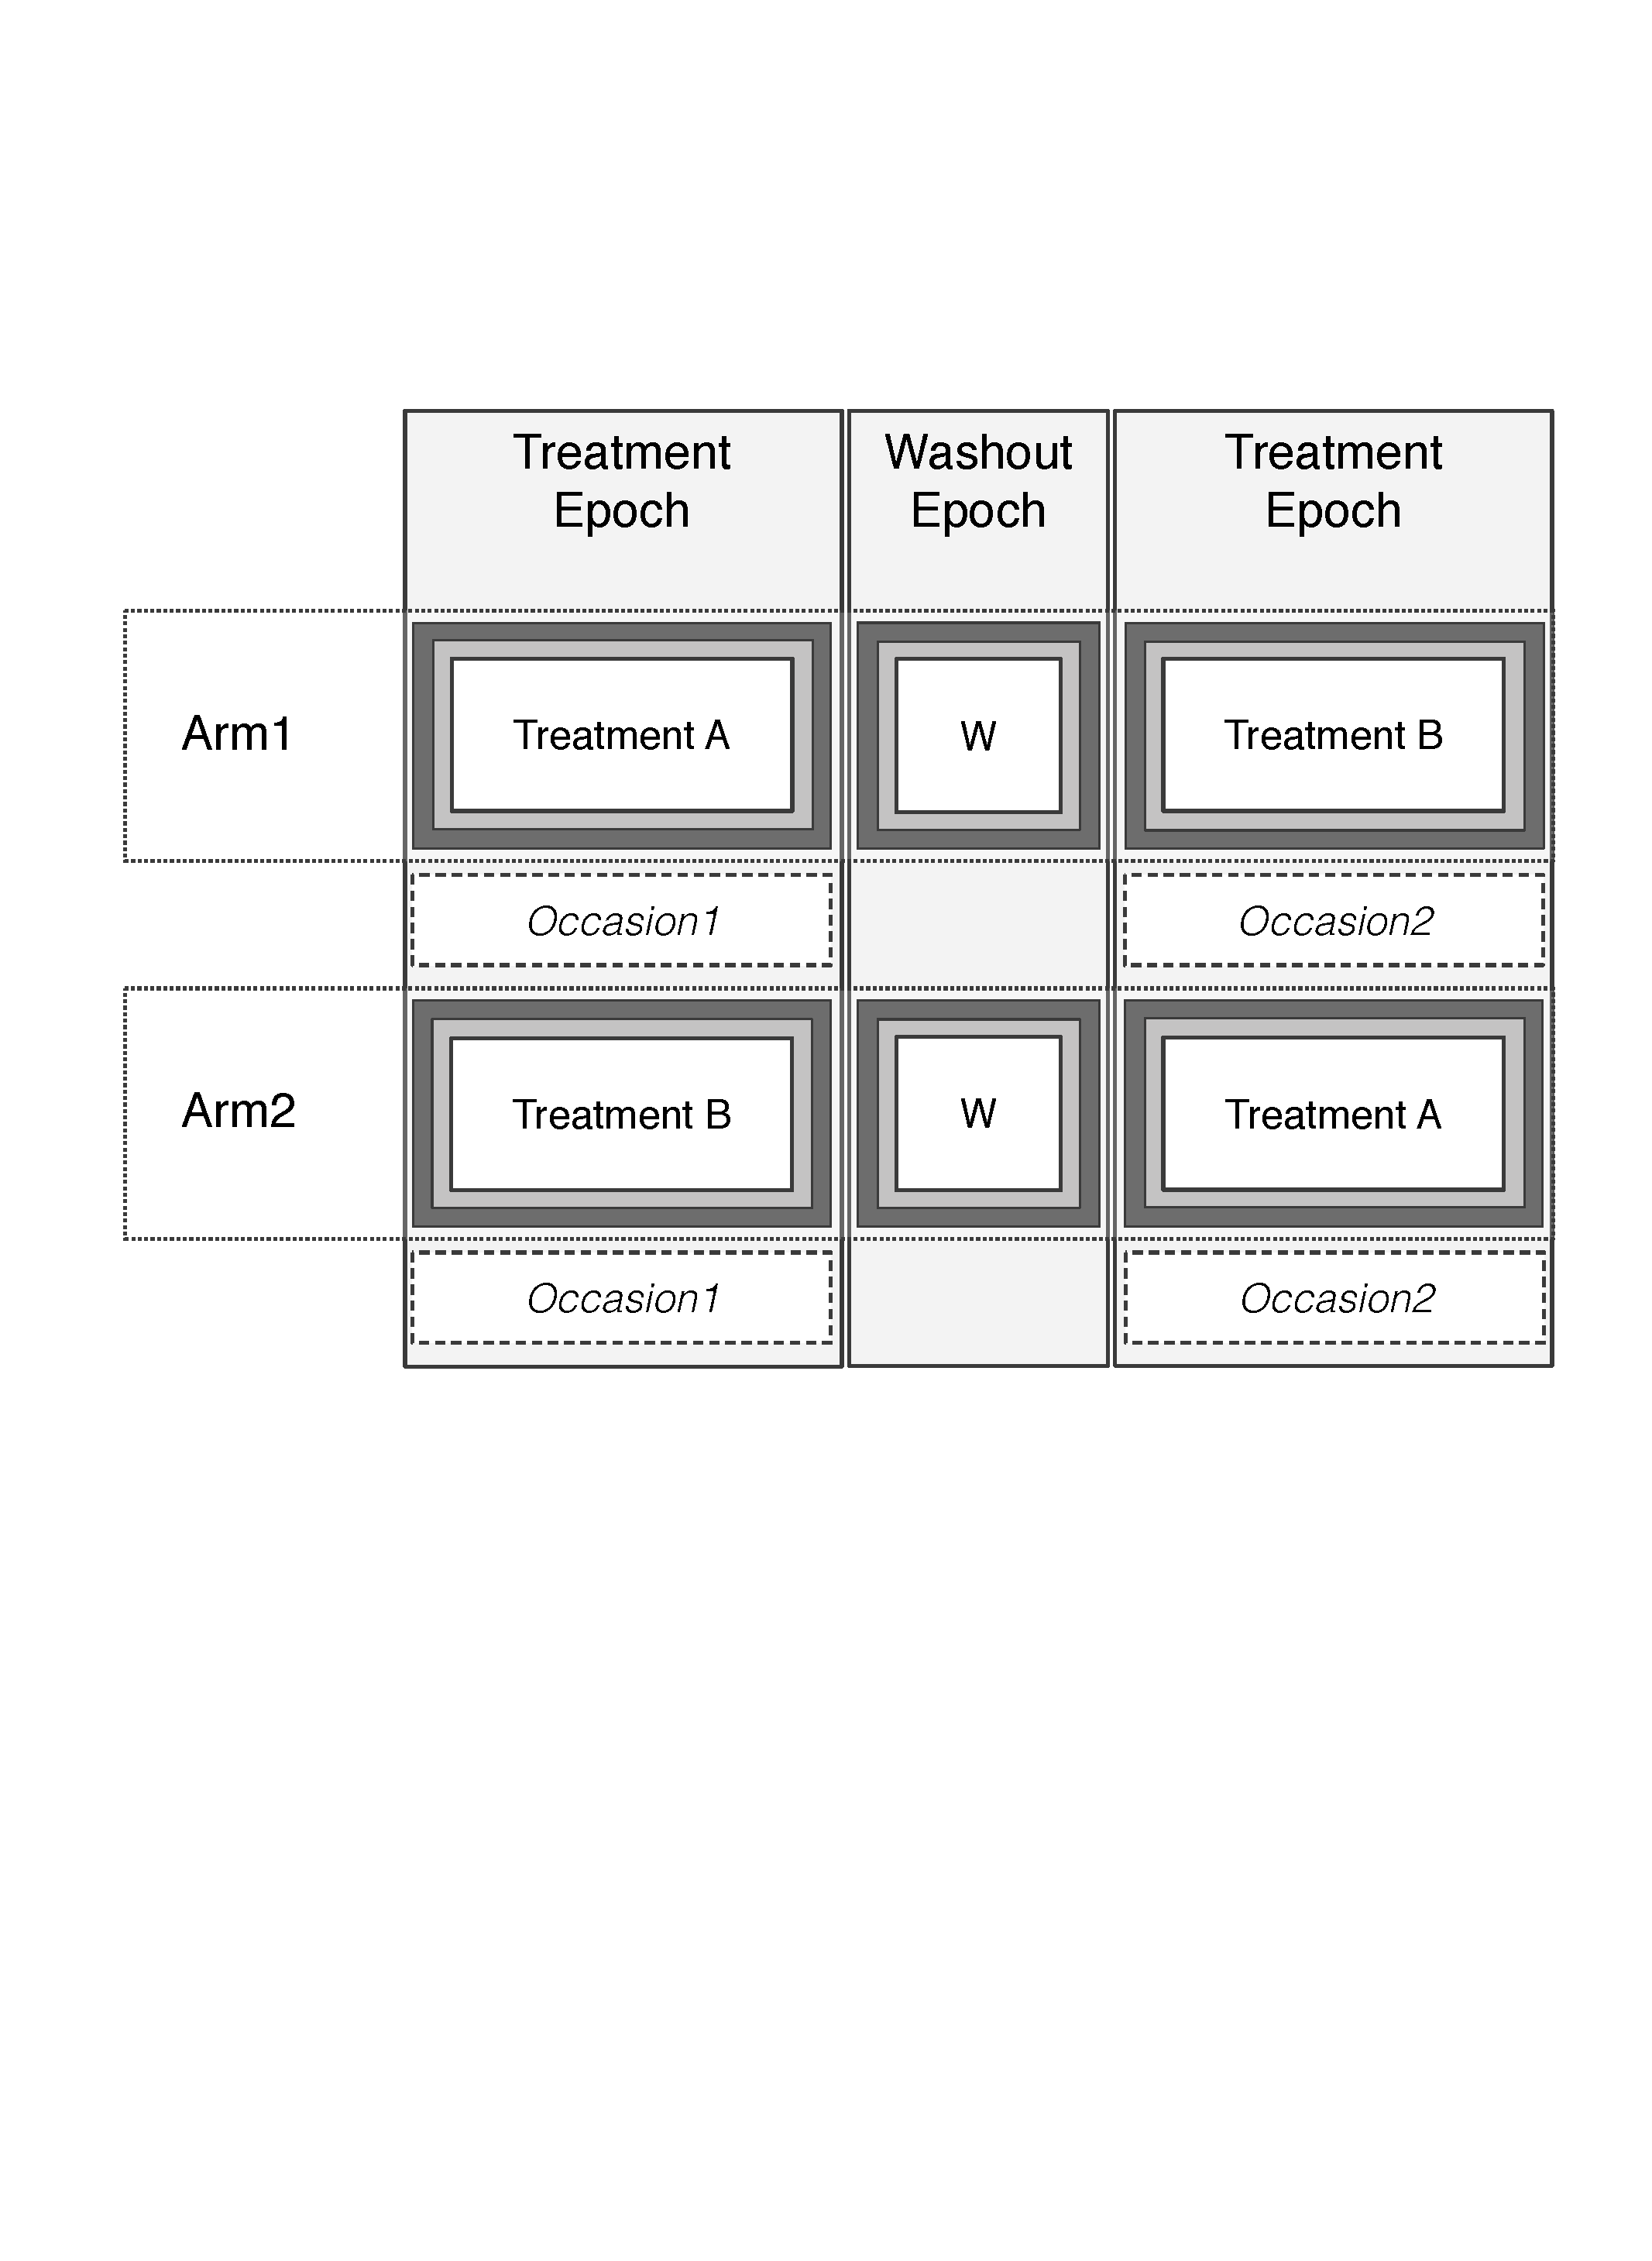
\includegraphics[width=0.7\linewidth]{pics/TwoArmsThreeEpochs_withWashout.pdf}
\caption{Schematic representation of a crossover design with washout. 
%The reader is referred to Figure \ref{fig:templateTrialDesign} for the colour code used to identify the elements of a trial. 
See tables \ref{fig:eg4:segmentCellArmEpoch} 
and \ref{fig:eg4:epochDef} for the detailed definition of segments, cells, arms, epochs
and occasions in this example.}
\label{fig:TwoArmsThreeEpochs_withWashout}
\end{figure}

%\noindent
\begin{table}[h]
\begin{center}
\begin{tabular}{lrr}\toprule
Arm & \textbf{1} & \textbf{2} \\\midrule
Number of subjects & 33 & 33\\
Dose variable & \var{D} & \var{D} \\
Dosing Amount & 100 & 150 \\
Dose Units & $\mg$ & $\mg$  \\
Dose per kg & no & no \\
Dosing times (h) &  0 &  0 \\
\bottomrule
\end{tabular}
\end{center}
\caption{Arms overview with dosing specification.}
\label{tab:ArmOverview}
\end{table}


%%%%%%%%%%%%%%%%%%%%%%%%%%%%%%%%%%%%%%%%%%%%%%%%%%%%%%%%%%%%%%%%
\subsubsection{Trial Design}
The model features a basic crossover design (see Figure
\ref{fig:TwoArmsThreeEpochs_withWashout}) with washout period and inter-occasion
variability (IOV). There are two treatments and the subjects are
organised into two arms that start with a different treatment. In
between each treatment there is a washout period during which time the
drug is eliminated from each subject. 
In the model the occasions, provide a second level of variability -- 
IOV \index{variability!IOV} (see section \ref{sec:variabilityModel}).  
This is summarised in Figure \ref{fig:eg4-IOV_2levels} (see also the listing 
in section \ref{eg4:variabilityModel}, showing relevant code 
within the element \xelem{VariabilityModel}).

The model also uses covariates to model the variability within the
model and so the treatments, the sequence of treatments (i.e.\xspace treatments A, B or
B,A) and the occasion itself are described in the covariate section
below.

\begin{figure}[ht!]
\centering
 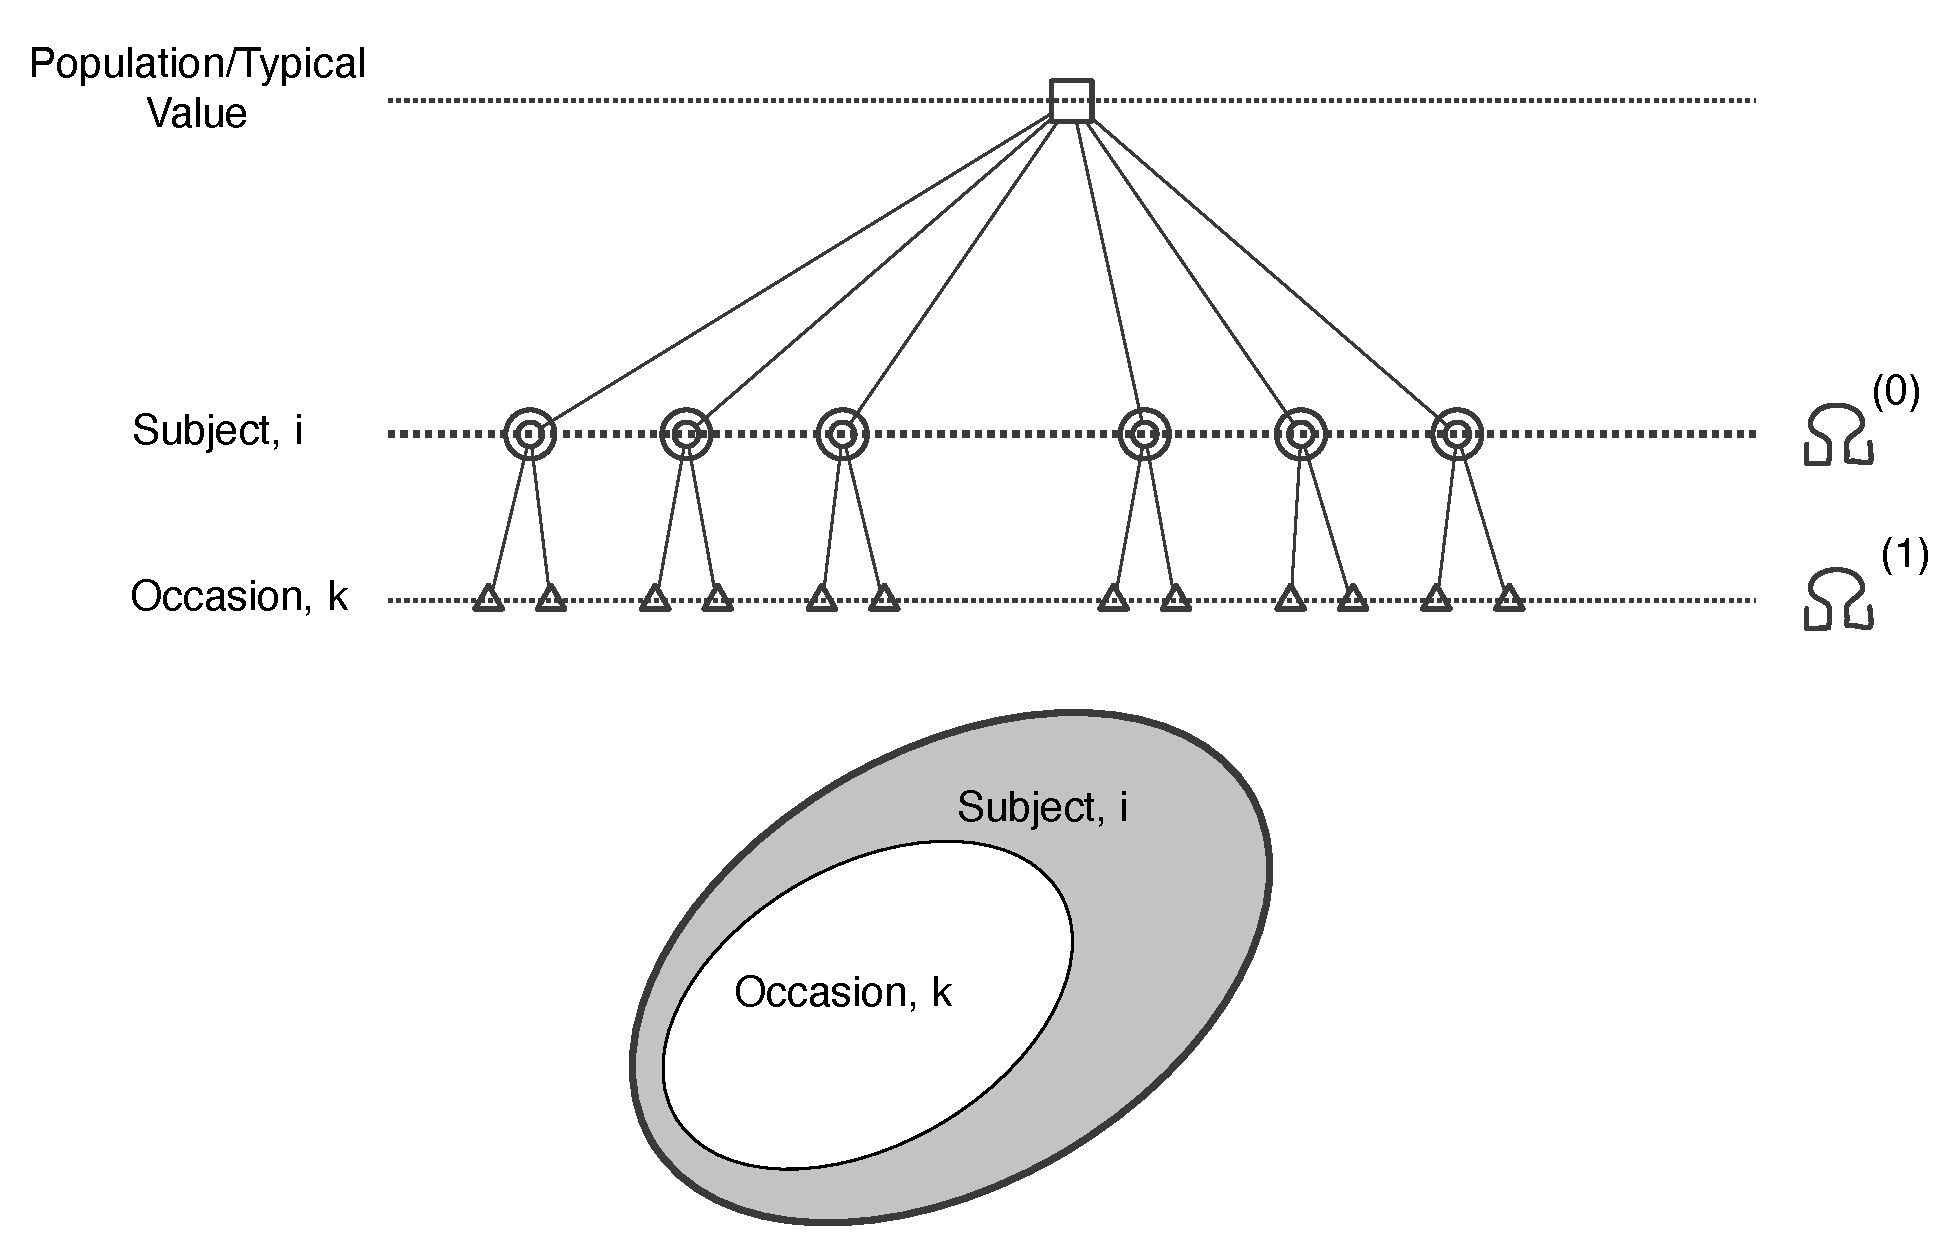
\includegraphics[width=120mm]{pics/IOV_2levels}
\caption{Two levels of variability -- inter-individual and inter-occasion within individual variability.}
\label{fig:eg4-IOV_2levels}
\end{figure}


%%%%%%%%%%%%%%%%%%%%%%%%%%%%%%%%%%%%%%%%%%%%%%%%%%%%%%%%%%%%%%%%
\subsubsection{Covariate Model}
\label{eg4:covariates-defn}

As discussed about all covariates are used to capture the explained variability in the model, 
see Table \ref{tab:CovariatesOverview}, and the \emph{Occasion} additionally
the unexplained expressed as the $\eta^{(+1)}$ random effects associated with CL and V.

\begin{table}[h]
\begin{center}
\begin{tabular}{lrrrr}\toprule
 & \textbf{Sex} &{\color{red}\textbf{Treat}}&{\color{mediumgreen}\textbf{TreatSeq}}&{\color{magenta}\textbf{Occasion}}\\\midrule
Type & Categorical & Categorical & Categorical & Categorical  \\
Category Count & 2 & 2 & 2 & 2\\
Categories & F, M & A, B & AB,BA & 1, 2\\
Reference & F & A & AB & 1\\
%Reference Probability & $14/36$ & 0.5  & 0.5  & 0.5\\
\bottomrule
\end{tabular}
\end{center}
\caption{Covariates overview.}
\label{tab:CovariatesOverview}
\end{table}

%%%%%%%%%%%%%%%%%%%%%%%%%%%%%%%%%%%%%%%%%%%%%%%%%%%%%%%%%%%%%%%%
\subsubsection{Parameter Model}

The parameter model includes random effects that represent the IIV and
{\color{lightblue}IOV} levels of variability. It also relates the
parameters to the covariates described above:
\begin{align}
\log(ka_{i}) &= \log(ka_{pop}) +
{\color{mediumgreen}\beta_{ka,TreatSeq}}1_{TreatSeq_i=AB} +
\eta_{ka,i} \label{eqn:eg4-param-ka}\\
\begin{split}
\log(V_{ik}) &= \log(V_{pop}) + {\boldsymbol \beta_V}1_{S_i=F} +
{\color{magenta}\beta_{V,OCC}} 1_{OCC_{ik}=1} \\
&\quad+ {\color{red}\beta_{V,Treat}}1_{Treat_{ik}=A} + {\color{mediumgreen}\beta_{V,TreatSeq}}1_{TreatSeq_i=AB} \\
		& \quad+ \eta_{V,i}^{(0)} +  {\color{lightblue} \eta_{V,ik}^{(+1)} }
\end{split} \label{eqn:eg4-parameter-v}\\
\begin{split}
\log(\CL_{ik}) &= \log(\CL_{pop}) + {\boldsymbol \beta_{\CL}}1_{S_i=F}
+ {\color{magenta}\beta_{\CL,OCC}} 1_{OCC_{ik}=1}\\
&\quad + \eta_{\CL,i}^{(0)} + {\color{lightblue} \eta_{Cl,ik}^{(+1)} }
\end{split}\nonumber
\end{align}
where
\begin{gather*}
\eta_{ka,i}^{(0)} \sim \mathcal{N}(0, \omega_{ka}), \quad \eta_{V,i}^{(0)} \sim \mathcal{N}(0, \omega_{V}), \quad \eta_{\CL,i}^{(0)} \sim \mathcal{N}(0, \omega_{\CL}),  \\
 {\color{lightblue} \eta_{V,ik}^{(+1)} \sim \mathcal{N}(0,\gamma_V)}, \quad
 {\color{lightblue} \eta_{\CL,ik}^{(+1)} \sim \mathcal{N}(0, \gamma_{\CL})}
\end{gather*}

The full variance-covariance matrices for our model read
\begin{gather}
 \Omega^{(0)} =
 \begin{pmatrix}
  \omega_{ka}^2 	& 0 				& 0  \\
   			  	& \omega_{V}^2	& 0 	\\
  				& 				& \omega_{\CL}^2\\
 \end{pmatrix}\label{eqn:eg4-covariance-mat}\\
 \Omega^{(+1)} =
 \begin{pmatrix}
0 & 0 & 0\\
 & \gamma_{V}^2	& 0 	\\
 & & \gamma_{\CL}^2\\
 \end{pmatrix}\label{eqn:eg4-gamma-mat}
\end{gather}


%%%%%%%%%%%%%%%%%%%%%%%%%%%%%%%%%%%%%%%%%%%%%%%%%%%%%%%%%%%%%%%%
\subsubsection{Structural model}

The model is first order absorption with linear elimination. This is the equivalent to 
oral1\_1cpt\_kaVCl (model 8) from \cite[Appendix I]{Bertrand:2008}.


%%%%%%%%%%%%%%%%%%%%%%%%%%%%%%%%%%%%%%%%%%%%%%%%%%%%%%%%%%%%%%%%
\subsubsection{Observation model}

We apply a residual error models to the output variable \var{C}.

%\noindent
\begin{center}
\begin{tabular*}{0.6\textwidth}{@{\extracolsep{\fill}} >{\bfseries}l l}\toprule
Output Variable  & \textbf{\itshape C} \\\midrule
Observations Name & Concentration\\
Units & $\mg/l$ \\
Observations Type & Continuous \\
Residual Error Model & Combined \\
Error Model Parameters & $a = 0.1,\quad b=0.1$\\
\bottomrule
\end{tabular*}
\end{center}


%%%%%%%%%%%%%%%%%%%%%%%%%%%%%%%%%%%%%%%%%%%%%%%%%%%%%%%%%%%%%%%%
\subsubsection{Modelling Steps}
Compared to the last example, we have define here two tasks:
\begin{itemize}
\item Estimation of population paramaters.
\item Estimation of the individual parameters.
\end{itemize}

%%%%%%%%%%%%%%%%%%%%%%%%%%%%%%%%%%%%%%%%%%%%%%%%%%%%%%%%%%%%%%%%
\subsection{Trial Design}

We have summaries the dosing regimen and organisation of the trial
design below, see also Figure \ref{fig:TwoArmsThreeEpochs_withWashout}.

\begin{table}[htdp!]
\begin{center}
\begin{tabular}{ccccccc}
\hline
Segment&Activity & Treatment & DoseTime & DoseSize & Target Variable \\
\hline
TA& OR1 &  OR bolus & $0:12:72$ & 150 & D \\
TA& OR2 &  OR bolus & $0:24:72$ & 100 & D \\
\hline
\end{tabular}
\end{center}
\caption{Segment/activity overview.}
\label{fig:eg4:segmentCellArmEpoch}
\end{table}

\begin{table}[htdp!]
\begin{center}
\begin{tabular}{cccc}
\hline
Epoch & Occasion & Start time & End time \\
\hline
Treatment Epoch & OCC1 & 0 &  180  \\
Washout & -- & 0 &  10  \\
Treatment Epoch & OCC2 & 0 &  180  \\
\hline
\end{tabular}
\end{center}
\caption{Epoch and occasion definition.}
\label{fig:eg4:epochDef}
\end{table}


%%%%%%%%%%%%%%%%%%%%%%%%%%%%%%%%%%%%%%%%%%%%%%%%%%%%%%%%%%%%%%%%
\subsubsection{Structure}
The implementation of the treatments, in \pharmml we use the
\xelem{Activity} element, is different compared to the previous example. 
See Table \ref{fig:eg4:segmentCellArmEpoch} for the details. The difference
is that now we have one dose administered at multiple dosing time points 
instead of single time point. See the following listing 
%\inputxml{exp6_dosingTimes.xml}
\lstset{language=XML}
\begin{lstlisting}
            <Activity oid="d1">
                <Bolus>
                    <DoseAmount inputTarget="parameter">
                        <ct:SymbRef blkIdRef="sm1" symbIdRef="D"/>
                        <ct:Assign>
                            <ct:Real>150</ct:Real>
                        </ct:Assign>
                    </DoseAmount>
                    <DosingTimes>
                        <ct:SymbRef blkIdRef="sm1" symbIdRef="tD"/>
                        <ct:Assign>
                            <ct:Sequence>
                                <ct:Begin><ct:Real>0</ct:Real></ct:Begin>
                                <ct:StepSize><ct:Real>12</ct:Real></ct:StepSize>
                                <ct:End><ct:Real>72</ct:Real></ct:End>
                            </ct:Sequence>
                        </ct:Assign>
                    </DosingTimes>
                </Bolus>
            </Activity>
\end{lstlisting}

how one can describe it within the \xelem{DosingTimes} element using the \xelem{Sequence}
structure defining the start/end times and step size.

Table \ref{fig:eg4:epochDef} gives an overview of the \var{Epochs} and \var{Occasions} 
in this example. Here, the occasions overlap with the epochs, the start and end times 
are identical, this is not always the case, the occasions can span one or more epochs. 
The \var{Washout} epoch is given here with start/end times as well which is in fact 
a redundant piece of information (but required by construction of an \var{Epoch})
as a \var{Washout} always assumes total reset of all drug amounts. 

As discussed in the section \ref{subsec:TrialStructure}, in \xelem{Structure} block 
we encode the variability which is located below the subject (see the 
hierarchy of the random variability discussed in section \ref{sec:variabilityModel}).
We call it the \textit{inter-occasion variability}, IOV. The following listing 
%\inputxml{exp6_structure_part3.xml} 
\lstset{language=XML}
\begin{lstlisting}
            <ObservationsEvent oid="occasions"> 
                <ArmRef oidRef="a1"/>
                <ArmRef oidRef="a2"/>
                <ct:VariabilityReference>
                    <ct:SymbRef blkIdRef="vm1" symbIdRef="iov1"/>
                </ct:VariabilityReference>
                <ObservationGroup oid="occ1">
                    <EpochRef oidRef="ep1"/>
                </ObservationGroup>
                <ObservationGroup oid="occ2">
                    <EpochRef oidRef="ep3"/>
                </ObservationGroup>
            </ObservationsEvent>
        </Structure>
\end{lstlisting}

shows how this is done. 
In this case the occasions coincide with the epochs 
so we use the \xelem{EpochRef} element. Alternatively, we could use the \xelem{Period}
element to define explicitly the start and end times of the occasions as shown 
in this listing: 
%\inputxml{exp6_structure_part4.xml}
\lstset{language=XML}
\begin{lstlisting}
            <!-- alternative -->
            <ObservationsEvent oid="occasions"> 
                <ArmRef oidRef="a1"/>
                <ArmRef oidRef="a2"/>
                <ct:VariabilityReference>
                    <ct:SymbRef blkIdRef="vm1" symbIdRef="iov1"/>
                </ct:VariabilityReference>
                <ObservationGroup oid="occ1">
                    <Period>
                        <Start><ct:Real>0</ct:Real></Start>
                        <End><ct:Real>180</ct:Real></End>
                    </Period>
                </ObservationGroup>
                <ObservationGroup oid="occ2">
                    <Period>
                        <Start><ct:Real>0</ct:Real></Start>
                        <End><ct:Real>180</ct:Real></End>
                    </Period>
                </ObservationGroup>
            </ObservationsEvent>
        </Structure>
\end{lstlisting}

This is of course very useful if the occasions do not
coincide with the epochs, or there are two or more occasions within one epoch.
In this case we set the \var{Start} and \var{End} times to $0$ and $180$, respectively.
These are exactly the same time points as are used in the epoch definition 
(see the first listing in section \ref{eg4_subsec:trialDesign} for how to encode epochs in the 
\xelem{Structure} definition).   


%%%%%%%%%%%%%%%%%%%%%%%%%%%%%%%%%%%%%%%%%%%%%%%%%%%%%%%%%%%%%%%%
\subsubsection{Population}
We pick up where we left off in the \xelem{Structure}, implementing
the hooks to the variability structure. The aspect we have not covered
yet is related to IIV.  The \xelem{Population} element is the place to
define any subject related variability and those levels above
it. The following listing shows how this works 
%\inputxml{exp6_population_part0.xml}
\lstset{language=XML}
\begin{lstlisting}
        <Population>
            <ct:VariabilityReference>
                <ct:SymbRef blkIdRef="vm1" symbIdRef="indiv"/>
            </ct:VariabilityReference>
            <!-- SKIP -->
\end{lstlisting}
In this example we deal only with the IIV and a level below it, so this is 
all we have to encode variability-wise at this point.

The next part of the \xelem{Population} block was discussed previously. 
Beside the standard assignment of subjects to an \var{Arm}
and providing information regarding \var{SEX}, we need to encode the information
about study design related covariates, see Table \ref{tab:CovariatesOverview}. 
Treatment type, \var{TREAT} which varies in this cross-over design as the study 
progress from \var{Epoch1} to \var{Epoch3}, is considered here as covariate.
And so are the treatment sequence, \var{TREATSEQ}, and occasions associated
with EPOCHs. 
This table is populated with data as can be seen in the following listing 
%\inputxml{exp6_population_part2.xml}
\lstset{language=XML}
\begin{lstlisting}
<ColumnMapping>
    <ds:ColumnRef columnIdRef="SEX"/>
    <ct:SymbRef blkIdRef="cm1" symbIdRef="Sex"/>
</ColumnMapping>
<ColumnMapping>
    <ds:ColumnRef columnIdRef="TREAT"/>
    <ct:SymbRef blkIdRef="cm1" symbIdRef="Treat"/>
</ColumnMapping>
<ColumnMapping>
    <ds:ColumnRef columnIdRef="TREATSEQ"/>
    <ct:SymbRef blkIdRef="cm1" symbIdRef="TreatSeq"/>
</ColumnMapping>
<ColumnMapping>
    <ds:ColumnRef columnIdRef="EPOCH"/>
    <ct:SymbRef symbIdRef="Occasion"/>
    <ds:CategoryMapping>
        <ds:Map dataSymbol="ep1" modelSymbol="occ1"/>
        <ds:Map dataSymbol="ep3" modelSymbol="occ2"/>
    </ds:CategoryMapping>
</ColumnMapping>
<ds:DataSet>
    <ds:Definition>
        <ds:Column columnId="ID" columnType="id" valueType="string" columnNum="1"/>
        <ds:Column columnId="ARM" columnType="arm" valueType="id" columnNum="2"/>
        <ds:Column columnId="SEX" columnType="covariate" valueType="string" columnNum="3"/>
        <ds:Column columnId="EPOCH" columnType="epoch" valueType="id" columnNum="4"/>
        <ds:Column columnId="TREAT" columnType="covariate" valueType="string" columnNum="5"/>
        <ds:Column columnId="TREATSEQ" columnType="covariate" valueType="string" columnNum="6"/>
    </ds:Definition>
    <ds:Table>
        <!-- arm1 -->
        <ds:Row><ct:String>1</ct:String><ct:Id>a1</ct:Id><ct:Id>M</ct:Id><ct:Id>ep1</ct:Id>
        											<ct:Id>A</ct:Id><ct:Id>AB</ct:Id></ds:Row>
        <ds:Row><ct:String>1</ct:String><ct:Id>a1</ct:Id><ct:Id>M</ct:Id><ct:Id>ep3</ct:Id>
        											<ct:Id>B</ct:Id><ct:Id>AB</ct:Id></ds:Row>
        <ds:Row><ct:String>2</ct:String><ct:Id>a1</ct:Id><ct:Id>M</ct:Id><ct:Id>ep1</ct:Id>
        											<ct:Id>A</ct:Id><ct:Id>AB</ct:Id></ds:Row>
        <ds:Row><ct:String>2</ct:String><ct:Id>a1</ct:Id><ct:Id>M</ct:Id><ct:Id>ep3</ct:Id>
        											<ct:Id>B</ct:Id><ct:Id>AB</ct:Id></ds:Row>
        <!-- arm2 -->
        <ds:Row><ct:String>9</ct:String><ct:Id>a2</ct:Id><ct:Id>M</ct:Id><ct:Id>ep1</ct:Id>
        											<ct:Id>B</ct:Id><ct:Id>BA</ct:Id></ds:Row>
        <ds:Row><ct:String>9</ct:String><ct:Id>a2</ct:Id><ct:Id>M</ct:Id><ct:Id>ep3</ct:Id>
        											<ct:Id>A</ct:Id><ct:Id>BA</ct:Id></ds:Row>
        <ds:Row><ct:String>10</ct:String><ct:Id>a2</ct:Id><ct:Id>M</ct:Id><ct:Id>ep1</ct:Id>
        											<ct:Id>B</ct:Id><ct:Id>BA</ct:Id></ds:Row>
        <ds:Row><ct:String>10</ct:String><ct:Id>a2</ct:Id><ct:Id>M</ct:Id><ct:Id>ep3</ct:Id>
        											<ct:Id>A</ct:Id><ct:Id>BA</ct:Id></ds:Row>
    </ds:Table>
</ds:DataSet>
</Population>
\end{lstlisting}
shows few subject data records for \var{Arm1} and \var{Arm2}. We have used 
in this example a new element, \xelem{CategoryMapping}, which use will be 
discussed in detail later in Section \ref{sec:eg4-NONMEMdataset}.


%%%%%%%%%%%%%%%%%%%%%%%%%%%%%%%%%%%%%%%%%%%%%%%%%%%%%%%%%%%%%%%%
\subsection{Variability Model}
\label{eg4:variabilityModel}

In this example the variability model is more complex than before, with IIV\index{variability!IIV} 
and IOV\index{variability!IOV} levels of variability, see Figure \ref{fig:eg4-IOV_2levels}. 
At this point in the \pharmml document we need to define the variability levels to be 
used in the rest of the document. You can see in the following listing 
%\inputxml{exp6_iov.xml}
\lstset{language=XML}
\begin{lstlisting}
        <VariabilityModel blkId="vm1" type="parameterVariability">
            <Level referenceLevel="true" symbId="indiv"/>
            <Level symbId="iov1">
                <ParentLevel>
                    <ct:SymbRef symbIdRef="indiv"/>
                </ParentLevel>
            </Level>
        </VariabilityModel>
\end{lstlisting}

that this is done by listing the variability levels using the \xelem{VariabilityLevel} 
element and their relationship. There are few important points to note here:
\begin{enumerate}
\item 
If more then one variability levels is used/defined in a model, it is useful to specify 
the reference level explicitly using the attribute \xatt{referenceLevel="true"} as can be seen
for the level called \xatt{indiv}. As explained previously it is not strictly required when
the dataset and column mapping are exhaustively defined but it simplifies the 
understudying of the variability model structure.
\item There is parent-child relationship between the levels of variability. The reference 
\var{Subject} level is referenced with the attribute \xatt{symbId="indiv"} is above the 
\var{Occasion} level, referenced with the attribute \xatt{symbId="iov1"} which is  
what is done using the \xelem{ParentLevel} in the listing.
\item The name given to a level, using the \xatt{symbId} attribute, is \textbf{not} 
significant. We used the names \var{iov1} and \var{indiv} to provide clarity in other 
parts of the example document.
\item The type of each variability level (e.g.,\xspace between-subject, inter-occasion, 
between-centre) is not defined here or in the Model Definition as a 
whole\footnote{N.B.,\xspace The numerical levels described in the variability 
model (section \ref{sec:variabilityModel}) are not used.}.
\end{enumerate}

In this example the \pharmml document tells us that there are two variability levels,
the reference \xatt{indiv} level and the lower level of variability is 
called ``\texttt{iov1}''\index{variability!IOV}\@. Moreover, we need to know their order 
relative to each other.


%%%%%%%%%%%%%%%%%%%%%%%%%%%%%%%%%%%%%%%%%%%%%%%%%%%%%%%%%%%%%%%%
\subsection{Covariate Model}

The covariate model describes categorical covariates, listed in Table 
\ref{tab:CovariatesOverview}, \index{covariate!categorical}which we have 
not seen in the previous examples. 

Because this is an estimation example no probabilities are provided and only the 
categories are defined, placed in the \xelem{Categorical} element. 
Then the implementation of each covariate follows the same
schema, which will be explained for the gender covariate \var{Sex}. 
There are obviously two categories the covariate can be associate with \textit{F} or \textit{M},
which are encoded using the \xelem{Category} element followed by an optional
\xelem{Name}. 

See the following listing how this is done 
%\inputxml{exp6_covariates.xml}
\lstset{language=XML}
\begin{lstlisting}
        <CovariateModel blkId="cm1">
            <Covariate symbId="Sex">
                <Categorical>
                    <Category catId="F">
                        <ct:Name>Female</ct:Name>
                    </Category>
                    <Category catId="M">
                        <ct:Name>Male</ct:Name>
                    </Category>
                </Categorical>
            </Covariate>
            <Covariate symbId="Treat">
                <Categorical>
                    <Category catId="A"/>
                    <Category catId="B"/>
                </Categorical>
            </Covariate>
            <Covariate symbId="TreatSeq">
                <Categorical>
                    <Category catId="AB">
                        <ct:Name>AB</ct:Name>
                    </Category>
                    <Category catId="BA">
                        <ct:Name>BA</ct:Name>
                    </Category>
                </Categorical>
            </Covariate>
            <Covariate symbId="Occasion">
                <Categorical>
                    <Category catId="occ1">
                        <ct:Name>1</ct:Name>
                    </Category>
                    <Category catId="occ2">
                        <ct:Name>2</ct:Name>
                    </Category>
                </Categorical>
            </Covariate>
        </CovariateModel>
\end{lstlisting}


%%%%%%%%%%%%%%%%%%%%%%%%%%%%%%%%%%%%%%%%%%%%%%%%%%%%%%%%%%%%%%%%
\subsection{Parameter Model}

In example \egref{1} (section \ref{sec:eg1}) we showed you how to define an individual
parameter in \pharmml and relate that to a continuous covariate. Now
in this example we will show how \pharmml can be used to describe
parameters that have multiple levels of variability and are related to
categorical covariates\index{covariate!categorical}.


In the following listing 
%\inputxml{exp6_ka.xml}
\lstset{language=XML}
\begin{lstlisting}
            <SimpleParameter symbId="omega_ka"/>
            <SimpleParameter symbId="pop_ka"/>
            <RandomVariable symbId="eta_ka">
                <ct:VariabilityReference>
                    <ct:SymbRef blkIdRef="vm1" symbIdRef="indiv"/>
                </ct:VariabilityReference>
                <NormalDistribution xmlns="http://www.uncertml.org/3.0" definition="">
                    <mean><rVal>0</rVal></mean>
                    <stddev><var varId="omega_ka"/></stddev>
                </NormalDistribution>
            </RandomVariable>
            <IndividualParameter symbId="ka">
                <GaussianModel>
                    <Transformation>log</Transformation>
                    <LinearCovariate>
                        <PopulationParameter>
                            <ct:Assign><ct:SymbRef symbIdRef="pop_ka"/></ct:Assign>
                        </PopulationParameter>
                        <Covariate>
                            <ct:SymbRef blkIdRef="cm1" symbIdRef="TreatSeq"/>
                            <FixedEffect>
                                <ct:SymbRef symbIdRef="beta_ka_treatseq"/>
                                <Category catId="AB"/>
                            </FixedEffect>
                        </Covariate>
                    </LinearCovariate>
                    <RandomEffects>
                        <ct:SymbRef symbIdRef="eta_ka"/>
                    </RandomEffects>
                </GaussianModel>
            </IndividualParameter>
\end{lstlisting}

 we show the definition of
parameter \var{ka}, which corresponds to (\ref{eqn:eg4-param-ka}). You
should be familiar with this structure by now, but you should take
note of the \xelem{Category} element within the \xelem{FixedEffect}
element. We use this to tell \pharmml that this fixed effect is related
to the ``\texttt{AB}'' category of the \var{TreatSeq} covariate. This
is equivalent to the expression
$\beta_{ka,TreatSeq}1_{TreatSeq_i=AB}$ in
(\ref{eqn:eg4-param-ka}). Note that it is possible to do this more
than once, for example if the covariate has more than two categories.


Parameter \var{ka} has only one level of variability, but this 
%\inputxml{exp6_V_part1.xml} 
\lstset{language=XML}
\begin{lstlisting}
            <SimpleParameter symbId="pop_V"/>
            <SimpleParameter symbId="omega_V"/>
            <SimpleParameter symbId="gamma_V"/>
            <SimpleParameter symbId="beta_V"/>
            <SimpleParameter symbId="beta_V_occ1"/>
            <SimpleParameter symbId="beta_V_Treat"/>
            <SimpleParameter symbId="beta_V_TreatSeq"/>
            <RandomVariable symbId="eta_V">
                <ct:VariabilityReference>
                    <ct:SymbRef blkIdRef="vm1" symbIdRef="indiv"/>
                </ct:VariabilityReference>
                <NormalDistribution xmlns="http://www.uncertml.org/3.0" definition="">
                    <mean><rVal>0</rVal></mean>
                    <stddev><var varId="omega_V"/></stddev>
                </NormalDistribution>
            </RandomVariable>
            <RandomVariable symbId="kappa_V">
                <ct:VariabilityReference>
                    <ct:SymbRef blkIdRef="vm1" symbIdRef="iov1"/>
                </ct:VariabilityReference>
                <NormalDistribution xmlns="http://www.uncertml.org/3.0" definition="">
                    <mean><rVal>0</rVal></mean>
                    <stddev><var varId="gamma_V"/></stddev>
                </NormalDistribution>
            </RandomVariable>
\end{lstlisting}

and this listing 
%\inputxml{exp6_V_part2.xml}
\lstset{language=XML}
\begin{lstlisting}
            <IndividualParameter symbId="V">
                <GaussianModel>
                    <Transformation>log</Transformation>
                    <LinearCovariate>
                        <PopulationParameter>
                            <ct:Assign><ct:SymbRef symbIdRef="pop_V"/></ct:Assign>
                        </PopulationParameter>
                        <Covariate>
                            <ct:SymbRef blkIdRef="cm1" symbIdRef="sex"/>
                            <FixedEffect>
                                <ct:SymbRef symbIdRef="beta_V"/>
                                <Category catId="F"/>
                            </FixedEffect>
                        </Covariate>
                        <Covariate>
                            <ct:SymbRef blkIdRef="cm1" symbIdRef="Occasion"/>
                            <FixedEffect>
                                <ct:SymbRef symbIdRef="beta_V_occ1"/>
                                <Category catId="occ1"/>
                            </FixedEffect>
                        </Covariate>
                        <Covariate>
                            <ct:SymbRef blkIdRef="cm1" symbIdRef="Treat"/>
                            <FixedEffect>
                                <ct:SymbRef symbIdRef="beta_V_Treat"/>
                                <Category catId="A"/>
                            </FixedEffect>
                        </Covariate>
                        <Covariate>
                            <ct:SymbRef blkIdRef="cm1" symbIdRef="TreatSeq"/>
                            <FixedEffect>
                                <ct:SymbRef symbIdRef="beta_V_TreatSeq"/>
                                <Category catId="AB"/>
                            </FixedEffect>
                        </Covariate>
                    </LinearCovariate>
                    <RandomEffects>
                        <ct:SymbRef symbIdRef="eta_V"/>
                    </RandomEffects>
                    <RandomEffects>
                        <ct:SymbRef symbIdRef="kappa_V"/>
                    </RandomEffects>
                </GaussianModel>
            </IndividualParameter>
\end{lstlisting}

show how we describe parameter
\var{V} with both IIV and IOV levels of variability. Very simply we
add a \xelem{RandomVariable} for each level of variability and use
the \xatt{symbIdRef} attribute in the \xelem{RandomEffects} element 
to map the random effect to the appropriate variability model as defined at 
the beginning of the \xelem{ModelDefinition} element. 
Thus \var{eta\_V} and \var{kappa\_V} correspond to the 
random effects $\eta^{(0)}_{V,i}$ and $\eta^{(+1)}_{V,ik}$ in
(\ref{eqn:eg4-parameter-v}). This parameter is related to all four
covariates, but we only show the \var{Sex} covariate. The others
defined in a very similar manner as all the covariates in this model
contain just 2 categories.

%%% TODO
We will not show parameter \var{Cl} as it does not illustrate any new
concepts, nor are any of the random effects in the model
correlated. This does not mean there is no covariance matrix defined
within the \pharmml document. There is. The matrices in
(\ref{eqn:eg4-covariance-mat}) and (\ref{eqn:eg4-gamma-mat}) are
implicitly defined because the standard deviations of the random effects 
are explicitly defined and no correlation between them is defined.


%%%%%%%%%%%%%%%%%%%%%%%%%%%%%%%%%%%%%%%%%%%%%%%%%%%%%%%%%%%%%%%%
\subsection{NONMEM dataset}
\label{sec:eg4-NONMEMdataset}
Now we will describe the case when the data and trial design are sourced from the 
NONMEM dataset. Table \ref{tab:example4_dataSet} show a typical dataset required for 
an estimation task.
\begin{table}[htdp]
\begin{center}
\small
\begin{tabular}{lllccccccc}\toprule
ID	& TIME	& DV			& AMT	& OCC	& TREAT	& TREATSEQ	& SEX 	& MDV 	& EVID \\ \midrule
1	& 0		& .			& 100	& 1		& 1		& 12			& 0 		& 1		& 1 \\ 
1	& 0.25	& 2.1243964	& .		& 1		& 1		& 12			& 0 		& 0		& 0 \\ 
1	& 0.5	& 4.308573	& .		& 1		& 1		& 12			& 0 		& 0		& 0  \\ 
1	& 1		& 7.6059305	& .		& 1		& 1		& 12			& 0 		& 0		& 0  \\ 
1	& 2		& 6.9678311	& .		& 1		& 1		& 12			& 0 		& 0		& 0  \\ 
1	& 3.5	& 7.7741686	& .		& 1		& 1		& 12			& 0 		& 0		& 0  \\ 
...	& ...		& ...			& ...		& ...		&...		& ...			& ... 		& ...		& ...  \\
1	& 24		& 1.5194051	& .		& 1		& 1		& 12			& 0 		& 0		& 0  \\ 
1	& 0		& .			& 100	& 2		& 2		& 12			& 0 		& 0		& 0  \\ 
1	& 0.25	& 4.2049182	& .		& 2		& 2		& 12			& 0 		& 0		& 0  \\ 
1	& 0.5	& 7.2508737	& .		& 2		& 2		& 12			& 0 		& 0		& 0  \\ 
1	& 1		& 8.5792413	& .		& 2		& 2		& 12			& 0 		& 0		& 0  \\ 
1	& 2		& 8.5689542	& .		& 2		& 2		& 12			& 0 		& 0		& 0  \\ 
1	& 3.5	& 10.1764867	& .		& 2		& 2		& 12			& 0 		& 0		& 0  \\ 
...	& ...		& ...			& ...		& ...		&...		& ...			& ... 		& ...		& ...  \\
1	& 24		& 0.8831267	& .		& 2		& 2		& 12			& 0 		& 0		& 0  \\ 
2	& 0		& .			& 100	& 1		& 2		& 21			& 1 		& 0		& 0  \\ 
2	& 0.25	& 2.6643053	& .		& 1		& 2		& 21			& 1 		& 0		& 0  \\ 
...	& ...		& ...			& ...		& ...		&...		& ...			& ... 		& 0		& 0  \\ \bottomrule
\end{tabular}
\end{center}
\caption{A dataset used in example \theexamples.}
\label{tab:example4_dataSet}
\end{table}%
and the following code shows how the according dataset definition and column mappings 
\lstset{language=XML}
\begin{lstlisting}
        <ExternalDataSet toolName="NONMEM" oid="NMoid">
            <ColumnMapping>
                <ds:ColumnRef columnIdRef="ID"/>
                <ct:SymbRef blkIdRef="vm1" symbIdRef="indiv"/>
            </ColumnMapping>
            <ColumnMapping>
                <ds:ColumnRef columnIdRef="Time"/>
                <ct:SymbRef symbIdRef="t"/>
            </ColumnMapping>
            <ColumnMapping>
                <ds:ColumnRef columnIdRef="Y"/>
                <ct:SymbRef blkIdRef="om1" symbIdRef="Cc_obs"/>
            </ColumnMapping>
            <ColumnMapping>
                <ds:ColumnRef columnIdRef="AMT"/>
                <ct:SymbRef blkIdRef="sm1" symbIdRef="D"/>
            </ColumnMapping>
            <!-- mapping occasions column to the covariate model -->
            <ColumnMapping>
                <ds:ColumnRef columnIdRef="OCC"/>
                <ct:SymbRef blkIdRef="cm1" symbIdRef="Occasion"/>
                <ds:CategoryMapping>
                    <ds:Map modelSymbol="occ1" dataSymbol="1"/>
                    <ds:Map modelSymbol="occ2" dataSymbol="2"/>
                </ds:CategoryMapping>
            </ColumnMapping>
            <!-- mapping occasions column to the variability model -->
            <ColumnMapping>
                <ds:ColumnRef columnIdRef="OCC"/>
                <ct:SymbRef blkIdRef="vm1" symbIdRef="iov1"/>
            </ColumnMapping>
            <ColumnMapping>
                <ds:ColumnRef columnIdRef="TREAT"/>
                <ct:SymbRef blkIdRef="cm1" symbIdRef="Treat"/>
                <ds:CategoryMapping>
                    <ds:Map dataSymbol="1" modelSymbol="A"/>
                    <ds:Map dataSymbol="2" modelSymbol="B"/>
                </ds:CategoryMapping>
            </ColumnMapping>
            <ColumnMapping>
                <ds:ColumnRef columnIdRef="TREATSEQ"/>
                <ct:SymbRef blkIdRef="cm1" symbIdRef="TreatSeq"/>
                <ds:CategoryMapping>
                    <ds:Map dataSymbol="12" modelSymbol="AB"/>
                    <ds:Map dataSymbol="21" modelSymbol="BA"/>
                </ds:CategoryMapping>
            </ColumnMapping>
            <ColumnMapping>
                <ds:ColumnRef columnIdRef="SEX"/>
                <ct:SymbRef blkIdRef="cm1" symbIdRef="Sex"/>
                <ds:CategoryMapping>
                    <ds:Map dataSymbol="0" modelSymbol="M"/>
                    <ds:Map dataSymbol="1" modelSymbol="F"/>
                </ds:CategoryMapping>
            </ColumnMapping>
            
            <!-- map 'tD' and 'TIME' if 'AMT' != 0 -->
            <ColumnMapping>
                <ds:ColumnRef columnIdRef="TIME"/>
                <ds:Piecewise>
                    <math:Piece>
                        <ct:SymbRef blkIdRef="sm1" symbIdRef="tD"/>
                        <math:Condition>
                            <math:LogicBinop op="neq">
                                <ds:ColumnRef columnIdRef="AMT"/>
                                <ct:Real>0</ct:Real>
                            </math:LogicBinop>
                        </math:Condition>
                    </math:Piece>
                </ds:Piecewise>
            </ColumnMapping>

            <ds:DataSet>
                <ds:Definition>
                    <ds:Column columnId="ID" columnType="id" valueType="string" columnNum="1"/>
                    <ds:Column columnId="TIME" columnType="time" valueType="real" columnNum="2"/>
                    <ds:Column columnId="Y" columnType="dv" valueType="real" columnNum="3"/>
                    <ds:Column columnId="AMT" columnType="dose" valueType="real" columnNum="4"/>
                    <ds:Column columnId="OCC" columnType="covariate" valueType="int" columnNum="5"/>
                    <ds:Column columnId="TREAT" columnType="covariate" valueType="int" columnNum="6"/>
                    <ds:Column columnId="TREATSEQ" columnType="covariate" valueType="int" columnNum="7"/>
                    <ds:Column columnId="SEX" columnType="covariate" valueType="int" columnNum="8"/>
                </ds:Definition>
                <ds:ImportData oid="dataOid">
                    <ds:path>example4.csv</ds:path>
                    <ds:format>CSV</ds:format>
                    <ds:delimiter>COMMA</ds:delimiter>
                </ds:ImportData>
            </ds:DataSet>
        </ExternalDataSet>
\end{lstlisting}
The mapping of the column \emph{OCC} deserves a short description. It is mapped twice
\begin{itemize}
\item
first, to map the occasions to the according covariate in \xelem{CovariateModel} \emph{cm1}
\item
second, to map them to the variability level, \xatt{iov1}, associated with the occasions defined
in the \xelem{VariabilityModel} \emph{vm1}
\end{itemize}
Compared to the previous examples the column mappings contain a new 
element, the \xelem{CategoryMapping} and within the \xelem{Map} elements 
use when mapping categorical covariates and discrete data model categories. 
Its attributes \xatt{dataSymbol} and \xatt{modelSymbol} identify the according 
symbols used in the model definition and the dataset, respectively.
 
Consider for example the covariate \emph{TREATSEQ}, in the model it is 
much more intuitive to use the \emph{AB} or \emph{BA} symbol id's then 
the corresponding 12 or 21 identifiers required as the NONMEM datasets 
are not allowing strings. The latter is also the reason why in this case we much
more often use the \xelem{ds:CategoryMapping} element as the dataset and model
use different symbols for the identical categories.

\subsection{Covered in previous examples}
The remaining elements of this example to be encoded in \pharmml
are nearly identical to those described before, such as \xelem{EstimationStep}
and \xelem{StepDepend\-encies} within the \xelem{ModellingSteps} block,
and will not be discussed here.

%%%%%%%%%%%%%%%%%%%%%%%%%%%%%%%%%%%%%%%%%%%%%%%%%%%%%%%%%%%%%%%%
%%%%%%%%%%%%%%%%%%%%%%%%%%%%%%%%%%%%%%%%%%%%%%%%%%%%%%%%%%%%%%%%
%%%%%%%%%%%%%%%%%%%%%%%%%%%%%%%%%%%%%%%%%%%%%%%%%%%%%%%%%%%%%%%%
\eglabel{5}
\section{Example \theexamples: Estimation with individual dosing}
\label{sec:Ribba}

%%%%%%%%%%%%%%%%%%%%%%%%%%%%%%%%%%%%%%%%%%%%%%%%%%%%%%%%%%%%%%%%
\subsection{Description}
This example is based on \cite{Ribba:2012uq} and deals with a mathematical
model describing the inhibition of the tumour growth of low-grade glioma treated
with chemotherapy\footnote{The example is encoded in two versions,  
\xatt{example5.xml} and \xatt{example5\_NONMEM.xml}, with explicit encoded trial 
design and design sourced from a NONMEM datafile, respectively.}. 
Although previous estimation examples were complex
enough to illustrate most important aspects of the current \pharmml specification 
we would like briefly to discuss this example due to its role as a use case. It also 
illustrates a new feature of the language, the fact that we can encode explicitly 
using patient specific administration scenarios within the \xelem{TrialDesign} section.

\begin{figure}[htbp]
\centering
\begin{tabular}{cc}
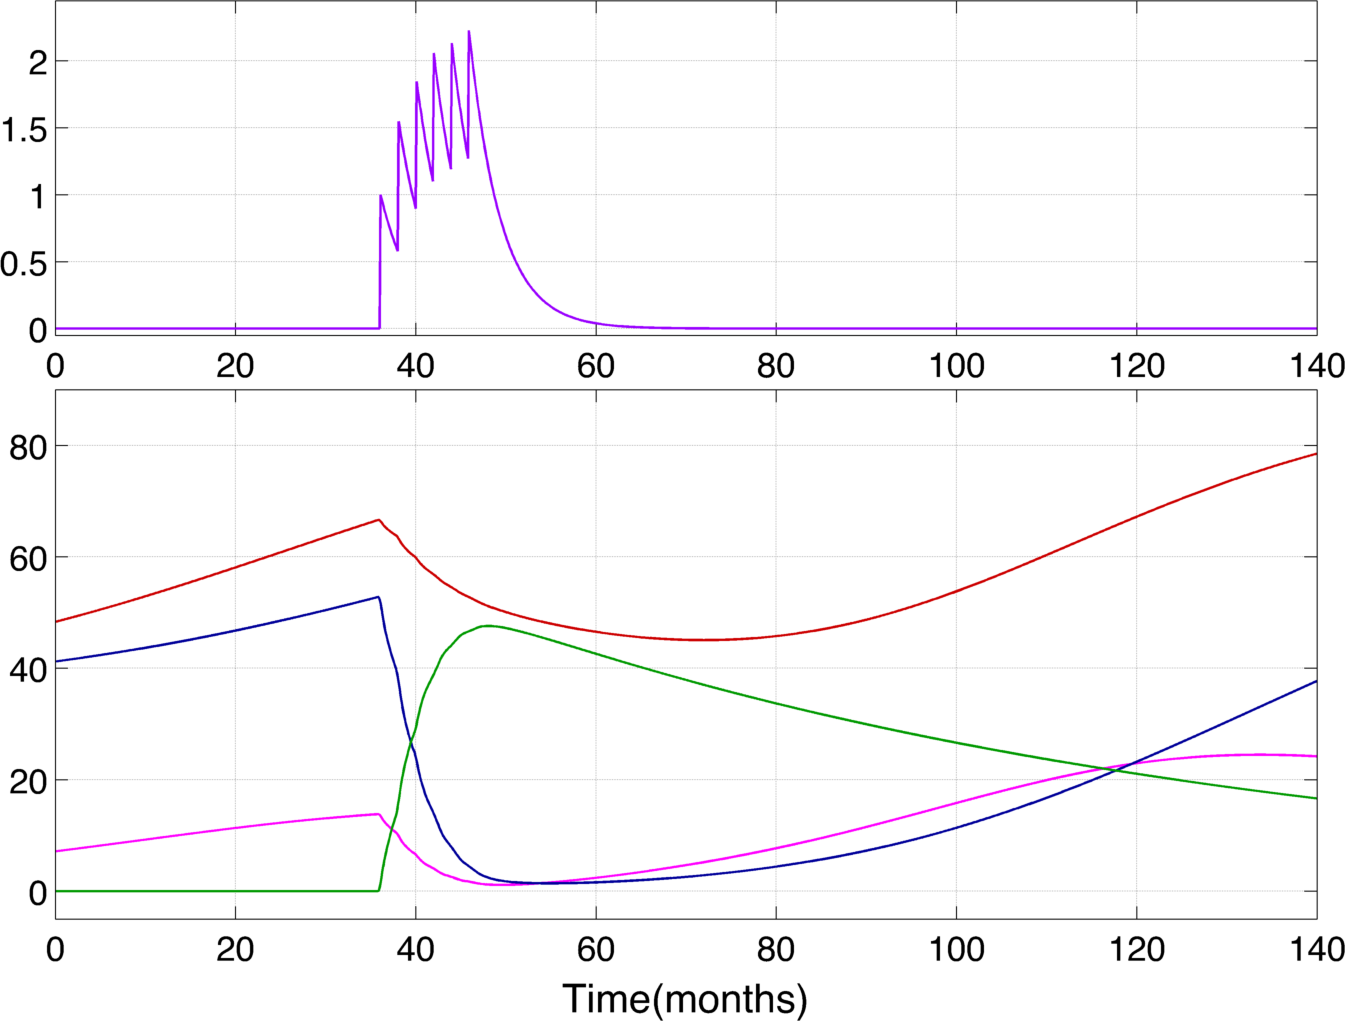
\includegraphics[width=.6\textwidth]{pics/example5_timeCourse} 
\end{tabular}
\caption{ (top) PK time course of the drug concentration, $C$. (bottom ) Tumour 
growth -- time courses for the total tumour size, $P^*$, and its components
 for one subject with dosing times = \{36.1, 38.05, 40.01, 41.96, 43.91, 45.87\}.}
\label{fig:oneSubjectPKandTumourGrowth}
\end{figure}

%%%%%%%%%%%%%%%%%%%%%%%%%%%%%%%%%%%%%%%%%%%%%%%%%%%%%%%%%%%%%%%%
\subsection{Trial design}
We will start with the definition of \xelem{Structure}, \xelem{Population}. The next language element, 
\xelem{IndividualDosing}, is, as mentioned above.

%%%%%%%%%%%%%%%%%%%%%%%%%%%%%%%%%%%%%%%%%%%%%%%%%%%%%%%%%%%%%%%%
\subsubsection{Structure}
Figure \ref{fig:1Arm1Epoch_RibbaDesign} shows the design structure of this example 
consisting of one arm and one epoch, meaning there is one treatment type 'IV' for all patients. 
As explained in section \ref{sec:CTS} the design element \xelem{Cell} comprises the 
essential elements specifying the information about the arm, epoch and segment/activities. 
\xelem{Segment} contains treatment definition, here an IV bolus administration, 
defined in the \xelem{Activity} element. 
%Figure \ref{fig:cellHierarchy_Ribba} shows 
%the general relationship of these elements (left) and how it applies to the current example (right).
See the following listing 
%\inputxml{Ribba_structure.xml}
\lstset{language=XML}
\begin{lstlisting}
        <Structure>
            <Epoch oid="epoch1">
                <Start><ct:Real>0</ct:Real></Start>
                <End><ct:Real>200</ct:Real></End>
                <Order>1</Order>
            </Epoch>
            <Arm oid="arm1"/>
            <Cell oid="cell1">
                <EpochRef oidRef="epoch1"/>
                <ArmRef oidRef="arm1"/>
                <SegmentRef oidRef="TA"/>
            </Cell>
            <Segment oid="TA">
                <ActivityRef oidRef="bolusIV"/>
            </Segment>
            <Activity oid="bolusIV">
                <Bolus>
                    <DoseAmount inputTarget="derivativeVariable">
                        <ct:SymbRef blkIdRef="sm1" symbIdRef="C"/>
                    </DoseAmount>
                </Bolus>
            </Activity>
        </Structure> 
\end{lstlisting}
for the PharmML implementation.

\begin{figure}[ht!]
\centering
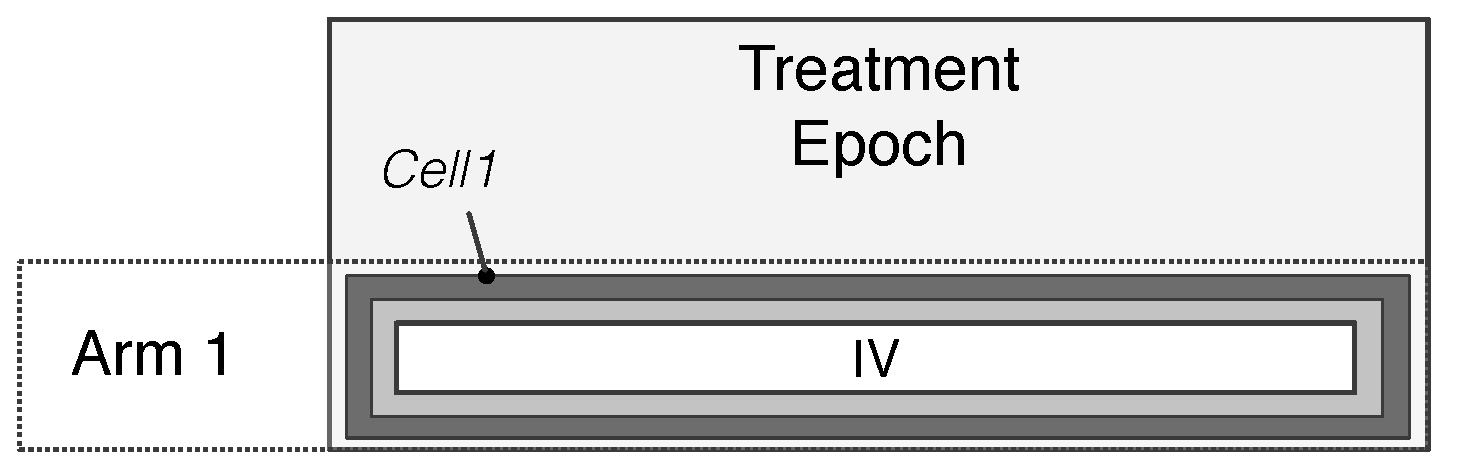
\includegraphics[width=0.7\linewidth]{pics/OneArmOneEpoch_IV}
\caption{Design overview: single arm design.}
\label{fig:1Arm1Epoch_RibbaDesign}
\end{figure}

%\begin{figure}[ht!]
%\centering
%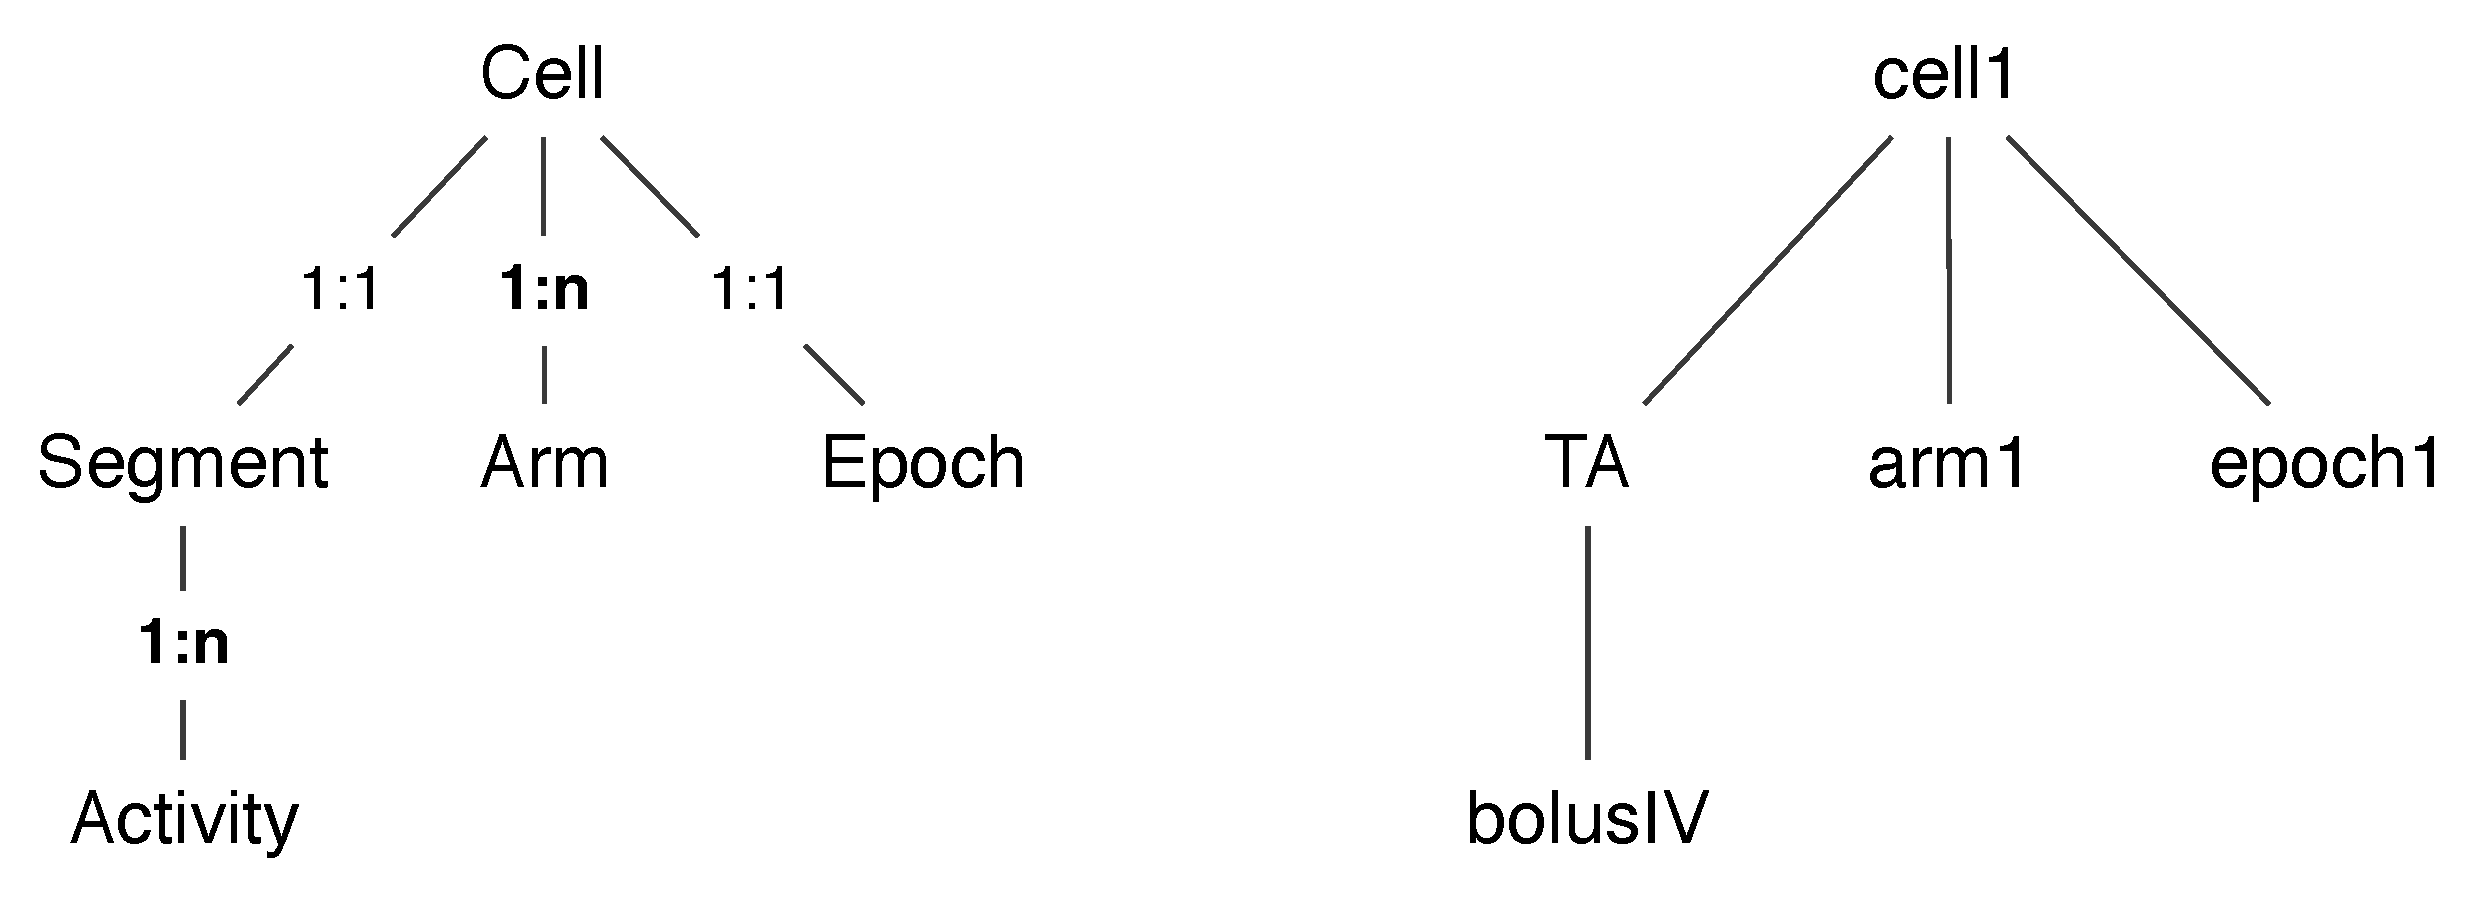
\includegraphics[width=0.7\linewidth]{pics/cellHierarchy_Ribba.pdf}
%\caption{General cell hierarchy (left); The root of the trial design structure hierarchy is the 'Cell' which can contain one 'Segment',
%one 'Epoch' and multiple 'Arms'. The 'Segment' element can have multiple child elements, the 'Activities', e.g. treatments or a washout. (right) An example of how it is applied in \cite{Ribba:2012uq}.}
%\label{fig:cellHierarchy_Ribba}
%\end{figure}

\begin{table}[htdp!]
\begin{center}
\begin{tabular}{ccccccc}
\hline
Segment&Activity & Treatment & DoseTime & DoseSize & Target Variable \\
\hline
TA& bolusIV &  IV bolus & individual & 1 & C \\
\hline
\end{tabular}
\end{center}
\caption{Segment/activity overview.}
\label{tab:segementActivity_Ribba}
\end{table}

%%%%%%%%%%%%%%%%%%%%%%%%%%%%%%%%%%%%%%%%%%%%%%%%%%%%%%%%%%%%%%%%
\subsubsection{Population}
In the next step, the \textit{Population} is defined, i.e. attributes of the individuals in the study. 
This means creating an individual template with columns for an identifier, arm and repetition and then
populating the table with appropriate data.
As no covariates are used here the \textit{Population} description reduces to the assignment 
of the subjects to the single study arm, \textit{Arm1}. As a shorthand we use the
\textit{repetition} method by defining the column 'rep', as can be seen in the following listing 
%\inputxml{Ribba_population.xml}
\lstset{language=XML}
\begin{lstlisting}
        <Population> 
            <ct:VariabilityReference>
                <ct:SymbRef blkIdRef="vm1" symbIdRef="indiv"/>
            </ct:VariabilityReference>
            
            <DataSet xmlns="http://www.pharmml.org/pharmml/0.6/Dataset">
                <Definition>
                    <Column columnId="ID" columnType="id" valueType="id" columnNum="1"/> 
                    <Column columnId="ARM" columnType="arm" valueType="id" columnNum="2"/> 
                    <Column columnId="REP" columnType="replicate" valueType="int" columnNum="3"/> 
                </Definition>
                <Table>
                    <Row>
                        <ct:Id>i</ct:Id>
                        <ct:Id>arm1</ct:Id>
                        <ct:Int>21</ct:Int>
                    </Row>
                </Table>
            </DataSet>
        </Population>
\end{lstlisting}

The identifiers, ID, created here are unique and will be used to the refer to specific subjects 
in the subsequent \xelem{IndividualDosing} structure element described in the following section.


%%%%%%%%%%%%%%%%%%%%%%%%%%%%%%%%%%%%%%%%%%%%%%%%%%%%%%%%%%%%%%%%
\subsubsection{Individual Dosing}
\label{subsubsec:Ribba_indivDosing}

This model utilises the idea of the so called K-PK model, meaning that the rate of the drug entry is relevant
but not its absolute value. Such models often assume, as it is the case here, that the dose is equal 1
for all subject and dosing events, see Table \ref{tab:example5_dataSet}.

The element \textit{IndividualDosing} is used to implementing all such subject specific
dosing events. First we have to associate the data which follow to an appropriate activity,
this is done by referring to the 'bolusIV' which defined previously in \xelem{Structure}, as 
as shown in the following listing 
%\inputxml{Ribba_individualDosing.xml}
\lstset{language=XML}
\begin{lstlisting}
        <IndividualDosing>
            <ActivityRef oidRef="bolusIV"/>
            <ColumnMapping>
                <ColumnRef xmlns="http://www.pharmml.org/pharmml/0.6/Dataset" columnIdRef="TIME"/>
                <ct:SymbRef symbIdRef="time"/>
            </ColumnMapping>
            <DataSet xmlns="http://www.pharmml.org/pharmml/0.6/Dataset">
                <Definition>
                    <Column columnId="ID" columnType="id" valueType="string" columnNum="1"/>
                    <Column columnId="TIME" columnType="idv" valueType="real" columnNum="2"/>
                    <Column columnId="DOSE" columnType="dose" valueType="real" columnNum="3"/>
                </Definition>
                <Table>
                    <!-- subject 1 -->
                    <Row><ct:String>1</ct:String><ct:Real>54.57</ct:Real><ct:Real>1</ct:Real></Row> 
                    <Row><ct:String>1</ct:String><ct:Real>59.77</ct:Real><ct:Real>1</ct:Real></Row> 
                    <!-- SNIP -->
                    <!-- subject 21 -->
                    <Row><ct:String>21</ct:String><ct:Real>1.5</ct:Real><ct:Real>1</ct:Real></Row> 
                    <Row><ct:String>21</ct:String><ct:Real>3.17</ct:Real><ct:Real>1</ct:Real></Row> 
                    <Row><ct:String>21</ct:String><ct:Real>4.85</ct:Real><ct:Real>1</ct:Real></Row> 
                    <Row><ct:String>21</ct:String><ct:Real>6.52</ct:Real><ct:Real>1</ct:Real></Row> 
                    <Row><ct:String>21</ct:String><ct:Real>8.19</ct:Real><ct:Real>1</ct:Real></Row> 
                    <Row><ct:String>21</ct:String><ct:Real>9.87</ct:Real><ct:Real>1</ct:Real></Row> 
                </Table>
            </DataSet>
        </IndividualDosing>
\end{lstlisting}

Next we map the subject's identifier \var{ID} to that created in the population definition. 
Finally a data set template using \xelem{Definition} element is defined, 
i.e. the columns \var{ID}, \var{TIME} and \var{DOSE}.
Then the table is populated with subject specific values as shown here for subjects 1, 2 and 21.


%%%%%%%%%%%%%%%%%%%%%%%%%%%%%%%%%%%%%%%%%%%%%%%%%%%%%%%%%%%%%%%%
\subsection{Structural model definition}
The following ODE system is defined:
\begin{align*}
\frac{dC}{dt} &= -\textit{KDE} \times C  \nonumber \\
\frac{dP}{dt} &= \lambda_P \times P \Big( 1 - \frac{P^\star}{K} \Big) + k_{\textit{QPP}} \times Q_P - k_{\textit{PQ}} \times P - \gamma \times C \times \textit{KDE} \times P  \nonumber \\
\frac{dQ}{dt} &= k_{PQ}\times P - \gamma \times C\times \mathit{KDE}\times Q \nonumber \\
\frac{dQ_P}{dt} &= \gamma \times C \times \textit{KDE} \times Q - k_{\textit{QPP}} \times Q_P - \delta_{\textit{QP}} \times Q_P  \nonumber \\ \nonumber \\
P^{\star} &= P + Q + Q_P \nonumber
\end{align*}
with initial conditions
\begin{align*}
C(t=0) = 1; \quad P(t=0) = P0; \quad Q(t=0) = Q0; \quad Q_P(t=0) = 0.  \nonumber
\end{align*}

%%%%%%%%%%%%%%%%%%%%%%%%%%%%%%%%%%%%%%%%%%%%%%%%%%%%%%%%%%%%%%%%
\subsubsection{Estimating initial conditions}
This example differs from the previous ones. It requires, in addition to model parameters, 
the estimation of the initial conditions of two tumour growth related variables. 
Moreover, the inter-individual variability is assumed for these variables.
The value for $Q_P(t=0)=Q_{P_0}$ is fixed to $0$ but the values for $P(t=0)=P_0$ and $Q(t=0)=Q_0$
are allowed to vary according to a log-normal distribution, see the following listing 
%\inputxml{Ribba_initialConditionsDef.xml} 
\lstset{language=XML}
\begin{lstlisting}
            <SimpleParameter symbId="pop_P0"/>
            <SimpleParameter symbId="omega_P0"/>
            <RandomVariable symbId="eta_P0">
                <ct:VariabilityReference>
                    <ct:SymbRef blkIdRef="vm1" symbIdRef="indiv"/>
                </ct:VariabilityReference>
                <NormalDistribution xmlns="http://www.uncertml.org/3.0" definition="">
                    <mean><rVal>0</rVal></mean>
                    <stddev><var varId="omega_P0"/></stddev>
                </NormalDistribution>
            </RandomVariable>
            <IndividualParameter symbId="P0">
                <GaussianModel>
                    <Transformation>log</Transformation>
                    <LinearCovariate>
                        <PopulationParameter>
                            <ct:Assign>
                                <ct:SymbRef symbIdRef="pop_P0"/>
                            </ct:Assign>
                        </PopulationParameter>
                    </LinearCovariate>
                    <RandomEffects>
                        <ct:SymbRef symbIdRef="eta_P0"/>
                    </RandomEffects>
                </GaussianModel>
            </IndividualParameter>            
\end{lstlisting}

where the definition of the distribution for the 
initial condition $P_0$ is shown.


%%%%%%%%%%%%%%%%%%%%%%%%%%%%%%%%%%%%%%%%%%%%%%%%%%%%%%%%%%%%%%%%
\subsection{NONMEM dataset}
\label{sec:eg5-NONMEMdataset}
Now we will describe the case when the data and trial design are sourced from the 
NONMEM dataset. Table \ref{tab:example4_dataSet} show a typical dataset required for 
an estimation task.
\begin{table}[htdp]
\begin{center}
\small
\begin{tabular}{rrrrrrrr}\toprule
ID	& TIME	& DV		& MDV	& AMT	& EVID \\ \midrule
1	& 0		& .		&  1		& .		& 0 \\
1	& 3.43	& 45.7	&  0		& .		& 0 \\
1	& 52.63	& 79.3	&  0		& .		& 0 \\
1	& 54.57	& .		&  1		& 1		& 1 \\
1	& 57.53	& 72.3	&  0		& .		& 0 \\
1	& 59.77	& .		&  1		& 1		& 1 \\
1	& 63.3	& 72.07	&  0		& .		& 0 \\
...	& ...		& ...		& ...		& ...		& ...  \\
1	& 121.87	& 90.16	&  0		& .		& 0 \\
2	& 0		& 50.17	&  0		& .		& 0 \\
2	& 12		& .		&  1		& 1		& 1 \\
2	& 14.09	& .		&  1		& 1		& 1 \\
2	& 14.17	& 52.82	&  0		& .		& 0 \\
...	& ...		& ...		& ...		& ...		& ... \\ \bottomrule
\end{tabular}
\end{center}
\caption{A dataset used in example \theexamples.
The columns are: the identifier, ID, time for measurements and dosing events, 
dependent variable, DV, which stands for \var{PSTAR} -- the total tumour size and 
the dose, DOSE. As common for K-PD models, the dose is equal 1 for all subjects and 
dosing events. }
\label{tab:example5_dataSet}
\end{table}%


The following code shows how the dataset definition and column mappings 
\lstset{language=XML}
\begin{lstlisting}
        <ExternalDataSet toolName="NONMEM" oid="NMoid">
            
            <ColumnMapping>
                <ColumnRef xmlns="http://www.pharmml.org/pharmml/0.6/Dataset" columnIdRef="ID"/>
                <ct:SymbRef blkIdRef="vm1" symbIdRef="indiv"/>
            </ColumnMapping>
            <ColumnMapping>
                <ColumnRef xmlns="http://www.pharmml.org/pharmml/0.6/Dataset" columnIdRef="TIME"/> 
                <ct:SymbRef symbIdRef="time"/>
            </ColumnMapping>
            <ColumnMapping>
                <ColumnRef xmlns="http://www.pharmml.org/pharmml/0.6/Dataset" columnIdRef="DV"/> 
                <ct:SymbRef blkIdRef="om1" symbIdRef="PSTAR_obs"/>
            </ColumnMapping>
            <ColumnMapping>
                <ColumnRef xmlns="http://www.pharmml.org/pharmml/0.6/Dataset" columnIdRef="AMT"/>
                <ct:SymbRef blkIdRef="om1" symbIdRef="C"/>
            </ColumnMapping>
            
            <!--columns: ID TIME DV MDV DOSE EVID-->
            <DataSet xmlns="http://www.pharmml.org/pharmml/0.6/Dataset">
                <Definition>
                    <Column columnId="ID" columnType="id" valueType="string" columnNum="1"/>
                    <Column columnId="TIME" columnType="time" valueType="real" columnNum="2"/>
                    <Column columnId="DV" columnType="dv" valueType="real" columnNum="3"/>
                    <Column columnId="MDV" columnType="mdv" valueType="int" columnNum="4"/>
                    <Column columnId="AMT" columnType="dose" valueType="real" columnNum="5"/>
                    <Column columnId="EVID" columnType="evid" valueType="int" columnNum="6"/>
                </Definition>
                <ImportData oid="dataOid">
                    <path>datasets/example5.csv</path>
                    <format>CSV</format>
                    <delimiter>COMMA</delimiter>
                </ImportData>
            </DataSet>
        </ExternalDataSet>
\end{lstlisting}


%%%%%%%%%%%%%%%%%%%%%%%%%%%%%%%%%%%%%%%%%%%%%%%%%%%%%%%%%%%%%%%%
\subsection{Modelling steps}
This requires the specification of the following items: \textit{EstimationStep} and \textit{StepDependencies}.
It has been described in previous examples in detail and will be skipped here.


%%%%%%%%%%%%%%%%%%%%%%%%%%%%%%%%%%%%%%%%%%%%%%%%%%%%%%%%%%%%%%%%
%%%%%%%%%%%%%%%%%%%%%%%%%%%%%%%%%%%%%%%%%%%%%%%%%%%%%%%%%%%%%%%%
%%%%%%%%%%%%%%%%%%%%%%%%%%%%%%%%%%%%%%%%%%%%%%%%%%%%%%%%%%%%%%%%

\eglabel{6}
\section{Example \theexamples: Joint PKPD model with count data}
\label{sec:eg6}
The following three examples features a new aspect of the \pml, the support of discrete 
data models\footnote{The discrete data models are coming in a large variety, which 
would be worth a detailed discussion. This and the next examples can cover, for 
the sake of space, only the very basic cases. More examples, encoded completely 
in \pml, can be found on our webpage \url{http://pharmml.org}. See also discrete data 
model templates in the appendix, \ref{chapter:codeTemplates}.}. The first one is using 
the Poisson distribution to describe count data\footnote{The example is encoded 
in \xatt{example6\_NONMEM.xml} with design sourced from a NONMEM datafile.}, 
from the MLXTRAN tutorial, \cite{Monolix4.3Tutorial:2014}.
%%%%%%%%%%%%%%%%%%%%%%%%%%%%%%%%%%%%%%%%%%%%%%%%%%%%%%%%%%%%%%%%
\subsection{Description}
\label{subsec:exp6_intro}
 
The essential bit of information for this task is the probability distribution, the probability 
mass function (PMF), of count data Y, which can be defined in either un-transformed, 
P(Y=k), or transformed, log(P(Y=k)), form. As in example \ref{sec:eg1}, the underlying 
PK model is 1-compartmental oral model and will be omitted here. We assume the basic 
Poisson model which reads
\begin{eqnarray}
&& P\big(Y_{\iijj}=k | \Cc_{\iijj}, \psi_i\big) =  \frac{e^{-\lambda_{\iijj}} \lambda^k_{\iijj}}{k!} \label{eq:poissonModel}
\end{eqnarray}
with concentration dependent mean $\lambda$, defined as
\begin{eqnarray}
&& \lambda_{\iijj} = \lambda_0 \Big(1 - \frac{\Cc_{\iijj}}{IC_{50} + \Cc_{\iijj}}\Big)  \label{eq:lambdasurface}
\end{eqnarray}
\begin{figure}[htbp]
\centering
%\begin{tabular}{cc}
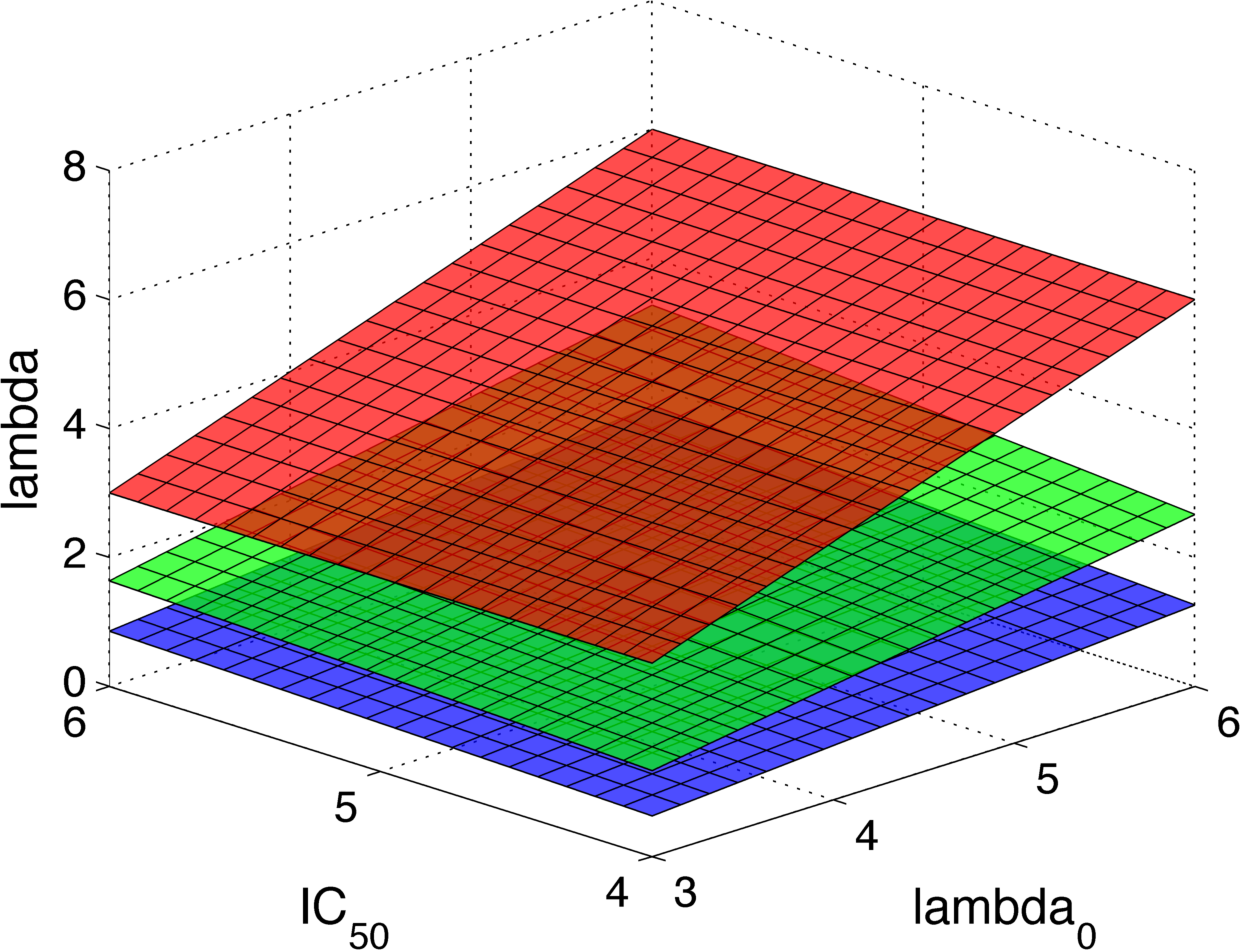
\includegraphics[width=.43\textwidth]{pics/CTS4_lambda_threeSurfaces} 
%& \raisebox{0\height}{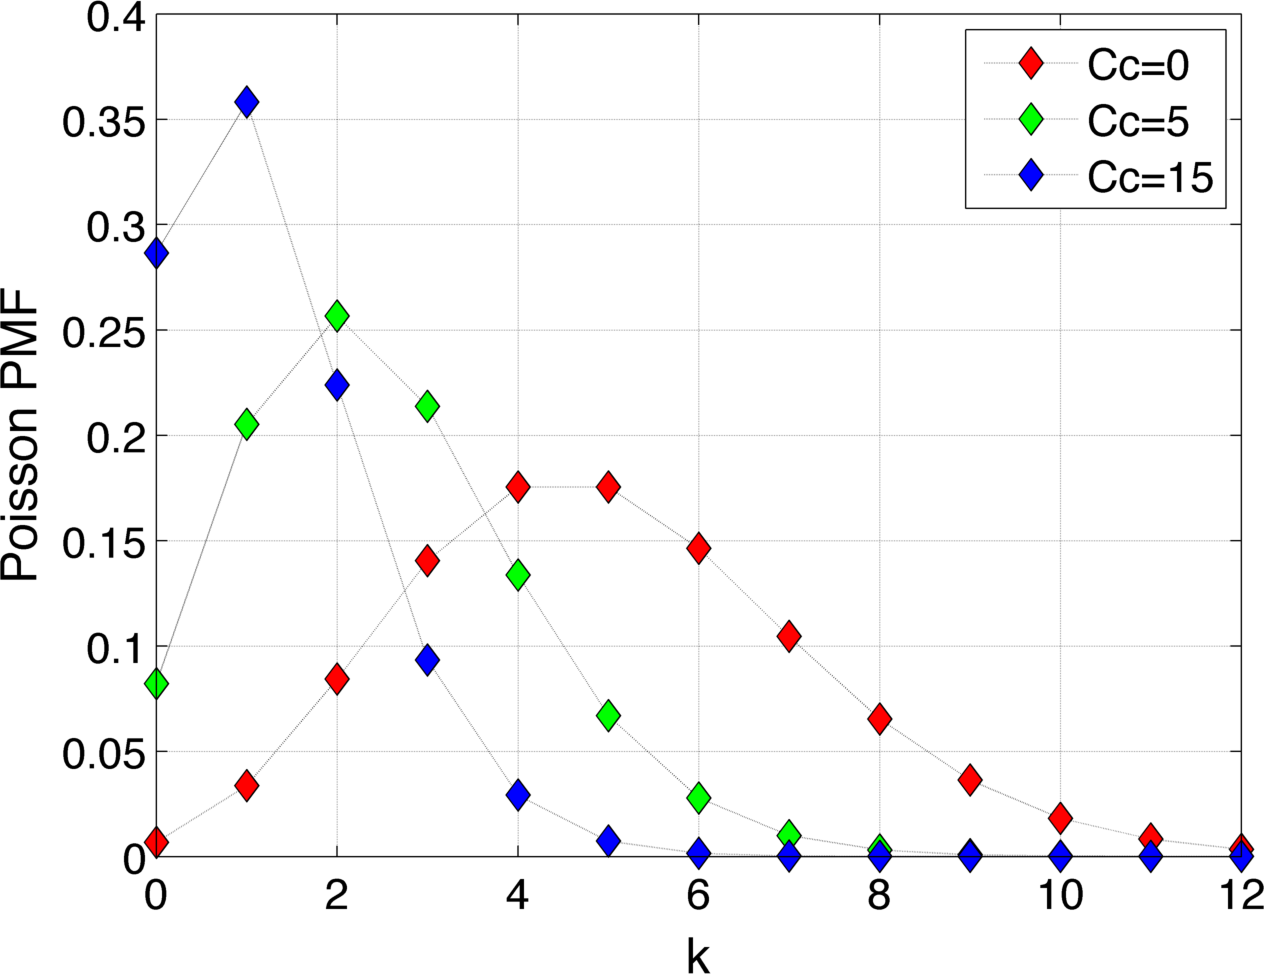
\includegraphics[scale=0.45]{pics/CTS4_poissonScan}}
%\end{tabular}
\caption{$\lambda$--surface as function of $\lambda_0$ and $IC_{50}$ 
plotted for $\Cc = \{1,5,15\}$.}
\label{fig:lambdasurface}
\end{figure}
also called \emph{Poisson intensity}. Here, $\lambda$, depends on the parameters 
$\lambda_0$ and $IC_{50}$ which are sampled from log-normal distribution. 
$\lambda_0$, stands here for the baseline seizure count prior to any drug. 
The value of $\lambda$ is reduced by the concentration in the central 
compartment, $\Cc$, which is visualised for three different values 
of $\Cc = \{1,5,15\}$ in \ref{fig:lambdasurface} ($1\equiv$ green, $5 \equiv$ 
red, $15 \equiv$ blue).


\begin{figure}[ht!]
\centering
\begin{tabular}{cc}
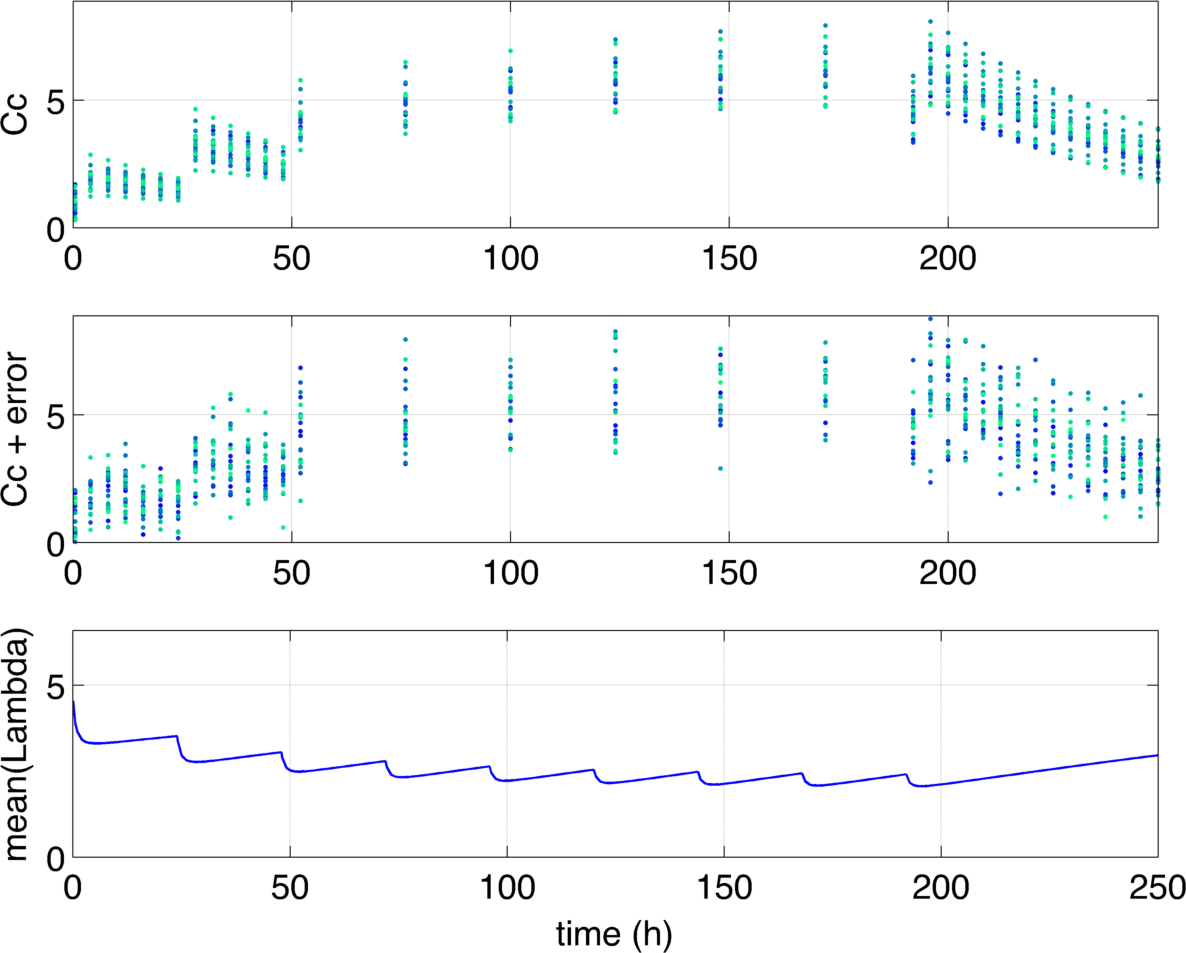
\includegraphics[width=.49\textwidth]{pics/CTS4_PK_meanLambda_armB} & 
\raisebox{0.05\height}{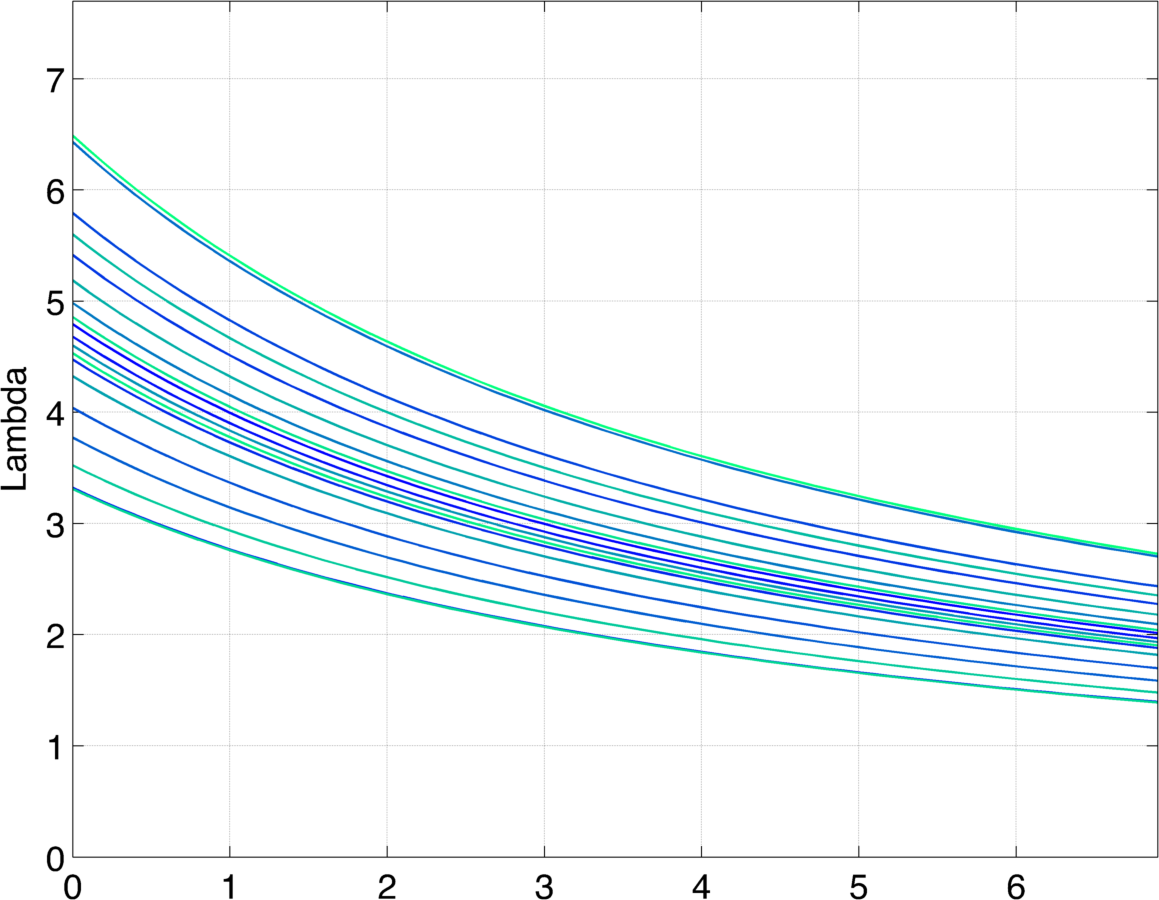
\includegraphics[scale=0.4875]{pics/CTS4_lambda}}
\end{tabular}
\caption{(left) The time courses for the concentration and mean Poisson intensity, $\lambda$. 
(right) Poisson intensity as given by eq.(\ref{eq:lambdasurface}) for all subject 
as function of the concentration between 0 and the maximum achievable 
concentration across 20 subjects.}
\label{fig:lambdaTiemCourse}
\end{figure}

\subsubsection{Individual parameters model}
\begin{eqnarray}
\lambda_0 & \sim&  \mbox{logNormal}(\pop_{\lambda_0}, \omega_{\lambda_0}); \quad  \pop_{\lambda_0} = 5, \quad \omega_{\lambda_0} = 0.2 \nonumber \\
IC_{50} &\sim& \mbox{logNormal}(\pop_{IC_{50}}, \omega_{IC_{50}}); \quad  \pop_{IC_{50}} = 5, \quad \omega_{IC_{50}} = 0 \nonumber
\end{eqnarray}


\subsubsection{Observation model}
We apply a combined residual error model to the continuous PK output variable 
\var{Cc} and Poisson error distribution for the discrete PD component, defined by \var{Y}, 
as the following table shows 

%\begin{table*}[h!]
\begin{center}
\small
\renewcommand{\arraystretch}{1.1}% 
\begin{tabular*}{0.8\linewidth}{@{\extracolsep{\fill}} >{\bfseries}l l l}\toprule
Output Variable & \textbf{\itshape Cc} &\textbf{\itshape Y}\\\midrule
Observation Name & Concentration & State \\
Units & $\mg/l$ & -- \\
Type & Continuous & Discrete/Count \\
Model & Combined & Poisson\\
Parameters 	& $a, b$ 	& $\lambda_0, IC_{50}$\\
%Regressor	& --		& $Cc$ \\
\bottomrule
\end{tabular*}
\end{center}
Two additional important bits of information which are part of the discrete observation
mode to be provided are 
\begin{itemize}
\item
Intensity Parameter, $\lambda$, given by eq. (\ref{eq:lambdasurface})
\item
Link function -- $\log$.
\end{itemize}

%%%%%%%%%%%%%%%%%%%%%%%%%%%%%%%%%%%%%%%%%%%%%%%%%%%%%%%%%%%%%%%%
\subsubsection{Modelling Steps}

The PK and PD output variables to be generated by the simulation and
their associated time points are shown below:

\begin{center}
\small
\renewcommand{\arraystretch}{1.1}% 
\begin{tabular*}{0.9\linewidth}{@{\extracolsep{\fill}} >{\bfseries}l c c}\toprule
Output Variable & \textbf{\itshape Cc} &\textbf{\itshape $\lambda$}\\\midrule
Observation times & [0.5,4 : 4 : 48, 52 : 24 : 192, 192 : 4 : 250] & 0 : 24 : 192\\
\bottomrule
\end{tabular*}
\end{center}


%%%%%%%%%%%%%%%%%%%%%%%%%%%%%%%%%%%%%%%%%%%%%%%%%%%%%%%%%%%%%%%%
\subsection{Observation model}
While the continuous observation model and its features as applied for example 
for the concentration have been described in very detail in the previous examples,
the error distribution of the discrete effect given by eqs.(\ref{eq:poissonModel}) 
and (\ref{eq:lambdasurface}) will be described in the following for the first time.

First we have to indicate the type of the observation model using the elements 
\xelem{Discrete} and specifically for this example the \xelem{CountData}. The next 
mandatory elements are the count index, \emph{k}, (required only when the PMF is 
explicitly specified, see below) and the \xelem{CountVariable} which will be used later
to establish the link between the model and the related date set, see Table 
\ref{tab:example6_dataSet}.
Then the characteristic parameter for the Poisson distribution is implemented, 
the \emph{Poisson intensity}, $\lambda$, as function of the drug concentration, $Cc$.

\lstset{language=XML}
\begin{lstlisting}
        <ObservationModel blkId="om1">
            <Discrete>
                <CountData>
                    <ct:Variable symbolType="int" symbId="k"/>
                    <CountVariable symbId="Y"/>
                    
                    <!-- Poisson intensity - function of drug concentration, Cc -->                    
                    <IntensityParameter symbId="Lambda">
                        <ct:Assign>
                            <math:Equation>
                                <math:Binop op="times">
                                    <ct:SymbRef blkIdRef="pm1" symbIdRef="lambda0"/>
                                    <math:Binop op="minus">
                                        <ct:Real>1</ct:Real>
                                        <math:Binop op="divide">
                                            <ct:SymbRef blkIdRef="sm1" symbIdRef="Cc"/>
                                            <math:Binop op="plus">
                                                <ct:SymbRef blkIdRef="pm1" symbIdRef="IC50"/>
                                                <ct:SymbRef blkIdRef="sm1" symbIdRef="Cc"/>
                                            </math:Binop>
                                        </math:Binop>
                                    </math:Binop>
                                </math:Binop>
                            </math:Equation>
                        </ct:Assign>
                    </IntensityParameter>
                    <!-- see next listing for the continuation of the observation model -->
\end{lstlisting}
Now the Poisson probability mass function (PMF) can be defined, but here 
in the transformed format 
\begin{align}
\log(P\big(Y_{\iijj} & =k | \Cc_{\iijj}, \psi_i\big)) =  -\lambda_{\iijj} +k\times \lambda_{\iijj} - \log(k!) \nonumber
\end{align}
which can be done in various ways, either
\begin{itemize}
\item
using the UncertML standard as in the following snippet
\lstset{language=XML}
\begin{lstlisting}
                    <PMF linkFunction="log">
                        <PoissonDistribution xmlns="http://www.uncertml.org/3.0" 
                            definition="http://www.uncertml.org/3.0">
                            <rate>
                                <var varId="Lambda"/>
                            </rate>
                        </PoissonDistribution>
                    </PMF>
                </CountData>
            </Discrete>
        </ObservationModel>
\end{lstlisting}
\item
by encoding explicitly the PMF in the transformed format and specifying the
the applied link function, here the logarithm, as the following snippet shows
\lstset{language=XML}
\begin{lstlisting}
                    <PMF linkFunction="log">
                        <math:LogicBinop op="eq">
                            <ct:SymbRef symbIdRef="Y"/>
                            <ct:SymbRef symbIdRef="k"/>
                        </math:LogicBinop>
                        <ct:Assign>
                            <Equation xmlns="http://www.pharmml.org/pharmml/0.6/Maths">
                                <Binop op="minus">
                                    <Binop op="plus">
                                        <Uniop op="minus">
                                            <ct:SymbRef symbIdRef="Lambda"/>
                                        </Uniop>
                                        <Binop op="times">
                                            <ct:SymbRef symbIdRef="k"/>
                                            <Uniop op="log">
                                                <ct:SymbRef symbIdRef="Lambda"/>
                                            </Uniop>
                                        </Binop>
                                    </Binop>
                                    <Uniop op="factln">
                                        <ct:SymbRef symbIdRef="k"/>
                                    </Uniop>
                                </Binop>
                            </Equation>
                        </ct:Assign>
                    </PMF>
                </CountData>
            </Discrete>
        </ObservationModel> 
\end{lstlisting}
\end{itemize}

Note, that although the UncertML driven solution is very simple and straightforward
to implement, it is also limited to only this case, see also Section \ref{subsec:DiscreteData}. 
In short, for count data models, only the basic Poisson model is available in the UncertML standard.


%%%%%%%%%%%%%%%%%%%%%%%%%%%%%%%%%%%%%%%%%%%%%%%%%%%%%%%%%%%%%%%%
\subsection{NONMEM dataset}
\label{sec:eg6-NONMEMdataset}
The remaining part is the the data and trial design as sourced from the 
NONMEM dataset. Table \ref{tab:example6_dataSet} show a typical dataset required for 
an estimation task.
\begin{table}[htdp]
\begin{center}
\small
\renewcommand{\arraystretch}{1.1}% 
\begin{tabular}{rrrrrrrr}\toprule
ID 	& TIME	& AMT	& Y		& DVID \\ \midrule
1 	& 0 		& 100 	& . 		& . \\ 
1 	& 4 		& . 		& 9.2 	& 1 \\ 
1 	& 8 		& . 		& 5 		& 2 \\ 
1 	& 12 	& . 		& 8.5 	& 1 \\ 
1 	& 18 	& . 		& 6.4 	& 1 \\ 
1 	& 24 	& . 		& 2 		& 2 \\ 
2 	& 0 		& 120	&  26 	& . \\ 
2 	& 4 		& . 		& 4.8 	& 1 \\ 
2 	& 8 		& . 		& 3 		& 2 \\ 
2 	& 12 	& . 		& 3.1 	& 1 \\ 
2 	& 18 	& . 		& 2.5 	& 1 \\ 
2 	& 24 	& . 		& 0 		& 2 \\ 
...	& ...		& ...		& ...		& ...	\\ \bottomrule
\end{tabular}
\end{center}
\caption{A dataset used in example for first two subjects.
The additional column DVID is used to specify the type of data. Here, 
DVID =1 is used for a continuous response and DVID =2 for count data.}
\label{tab:example6_dataSet}
\end{table}%

\lstset{language=XML}
\begin{lstlisting}
        <mstep:ExternalDataSet toolName="NONMEM" oid="NMoid">
            <mstep:ColumnMapping>
                <ds:ColumnRef columnIdRef="TIME"/>
                <ct:SymbRef symbIdRef="t"/>
            </mstep:ColumnMapping>
            <mstep:ColumnMapping>
                <ds:ColumnRef columnIdRef="AMT"/>
                <ct:SymbRef blkIdRef="sm1" symbIdRef="Ad"/>
            </mstep:ColumnMapping>
            <mstep:MultipleDVMapping>
                <ds:ColumnRef columnIdRef="DV"/>
                <mstep:Piecewise>
                    <math:Piece>
                        <ct:SymbRef blkIdRef="om1" symbIdRef="Y"/>
                        <math:Condition>
                            <math:LogicBinop op="eq">
                                <ds:ColumnRef columnIdRef="DVID"/>
                                <ct:Int>2</ct:Int>
                            </math:LogicBinop>
                        </math:Condition>
                    </math:Piece>
                    <math:Piece>
                        <ct:SymbRef blkIdRef="om2" symbIdRef="Cc_obs"/>
                        <math:Condition>
                            <math:LogicBinop op="eq">
                                <ds:ColumnRef columnIdRef="DVID"/>
                                <ct:Int>1</ct:Int>
                            </math:LogicBinop>
                        </math:Condition>
                    </math:Piece>
                </mstep:Piecewise>
            </mstep:MultipleDVMapping>
            <ds:DataSet>
                <ds:Definition>
                    <ds:Column columnId="ID" columnType="id" valueType="string" columnNum="1"/>
                    <ds:Column columnId="TIME" columnType="idv" valueType="real" columnNum="2"/>
                    <ds:Column columnId="AMT" columnType="dose" valueType="real" columnNum="3"/>
                    <ds:Column columnId="DV" columnType="dv" valueType="real" columnNum="4"/>
                    <ds:Column columnId="DVID" columnType="dvid" valueType="real" columnNum="5"/>
                </ds:Definition>
                <ds:ExternalFile oid="dataOid">
                    <ds:path>datasets/example_poisson.csv</ds:path>
                </ds:ExternalFile>
            </ds:DataSet>
        </mstep:ExternalDataSet>
\end{lstlisting}

Mapping of dosing related data has been described previously on
multiple occasions and will not be discussed here. The conditional mapping required 
in the case when multiple observations have to be mapped using the \xelem{mstep:MultipleDVMapping}
has been described in example 1, see section \ref{sec:eg1-NONMEMdataset}. 
What is new however is the mapping target when dealing with count data.
The count variable, \emph{Y}, as defined in the very beginning of the \xelem{CountData} 
in the observation model \xatt{om1} as the snippet shows
\lstset{language=XML}
\begin{lstlisting}
		<CountVariable symbId="Y"/>
\end{lstlisting}
is the target for this mapping and is conditional on the value of the column \emph{DVID}.




%%%%%%%%%%%%%%%%%%%%%%%%%%%%%%%%%%%%%%%%%%%%%%%%%%%%%%%%%%%%%%%%
%%%%%%%%%%%%%%%%%%%%%%%%%%%%%%%%%%%%%%%%%%%%%%%%%%%%%%%%%%%%%%%%
%%%%%%%%%%%%%%%%%%%%%%%%%%%%%%%%%%%%%%%%%%%%%%%%%%%%%%%%%%%%%%%%

\newpage

\eglabel{7}
\section{Example \theexamples: Joint PKPD model with categorical data}
\label{sec:eg7}

%%%%%%%%%%%%%%%%%%%%%%%%%%%%%%%%%%%%%%%%%%%%%%%%%%%%%%%%%%%%%%%%
\subsection{Description}
\label{subsec:exp7_intro} 
The following example features another type of discrete models supported by \pml -- 
the categorical data models.

In this example, there are two categories, $k \in {0,1}$, i.e. the effect outcome is either 0 or 1. 
The underlying PK model is again an 1-compartmental oral model and will no t be described. 
The probability for the category 1 is given by the following formula 
\begin{eqnarray}
	p1 &=& \frac{1}{1+\exp(-\theta_1 - \theta_2 \log(\Cc))} 	\label{eq:p1surface}
\end{eqnarray}
which is plotted in \ref{fig:p1surface}. This $p1$--surface is also function of $\theta_1$, 
$\theta_2$ and $log(\Cc)$ which is visualised for three different values of $\Cc = \{1,5,15\}$. 

\begin{figure}[htbp]
\begin{center}
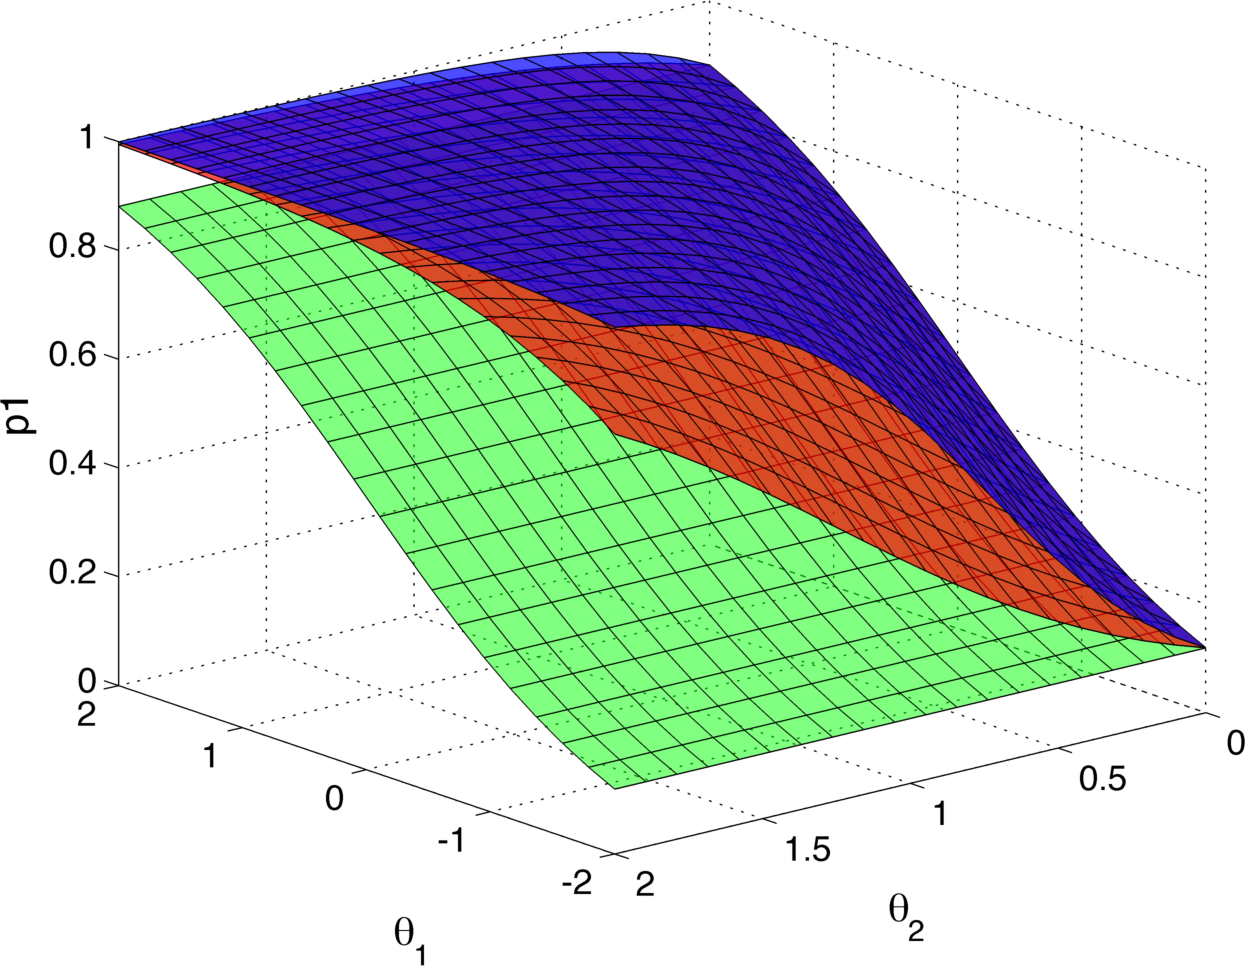
\includegraphics[width=.45\textwidth]{pics/p1_threeSurfaces.png}
\caption{p1 probability surface as function of $\theta_1$ and $\theta_2$ plotted for 
Cc = \{1,5,15\} ($1\equiv$ green, $5 \equiv$ red, $15 \equiv$ blue). }
\label{fig:p1surface}
\end{center}
\end{figure}

\subsubsection{Individual parameters model}
\begin{eqnarray}
theta1& \sim&  \mbox{Normal}(\pop_{theta1}, \omega_{theta1}); \quad \pop_{theta1}=-1,\quad \omega_{theta1}=0.3 \nonumber \\
theta2& \sim&  \mbox{logNormal}(\pop_{theta2}, \omega_{theta2}); \quad \pop_{theta2}=1,\quad \omega_{theta2}=0.2 \nonumber 
\end{eqnarray}

\subsubsection{Observation model}
We apply a combined residual error model to the continuous PK output variable 
\var{Cc} and Poisson error distribution for the discrete PD component, defined by \var{Y}, 
as the following table shows 

%\begin{table*}[h!]
\begin{center}
\small
\renewcommand{\arraystretch}{1.1}% 
\begin{tabular*}{0.8\linewidth}{@{\extracolsep{\fill}} >{\bfseries}l l l}\toprule
Output Variable & \textbf{\itshape Cc} &\textbf{\itshape Y}\\\midrule
Observation Name & Concentration & State \\
Units & $\mg/l$ & -- \\
Type & Continuous & Discrete/Categorical \\
Model & Combined & Binomial\\
Parameters 	& $a, b$ 	& $\theta_1$, $\theta_2$\\
%Regressor	& --		& $Cc$ \\
\bottomrule
\end{tabular*}
\end{center}

%%%%%%%%%%%%%%%%%%%%%%%%%%%%%%%%%%%%%%%%%%%%%%%%%%%%%%%%%%%%%%%%
\subsubsection{Modelling Steps}

The PK and PD output variables to be generated by the simulation and
their associated time points are shown below:

\begin{center}
\small
\renewcommand{\arraystretch}{1.1}% 
\begin{tabular*}{0.9\linewidth}{@{\extracolsep{\fill}} >{\bfseries}l c c}\toprule
Output Variable & \textbf{\itshape Cc} &\textbf{\itshape $p1$}\\\midrule
Observation times & [0.5,4 : 4 : 48, 52 : 24 : 192, 192 : 4 : 250] & 0 : 24 : 288\\
\bottomrule
\end{tabular*}
\end{center}


\begin{figure}[htbp]
\centering
\begin{tabular}{cc}
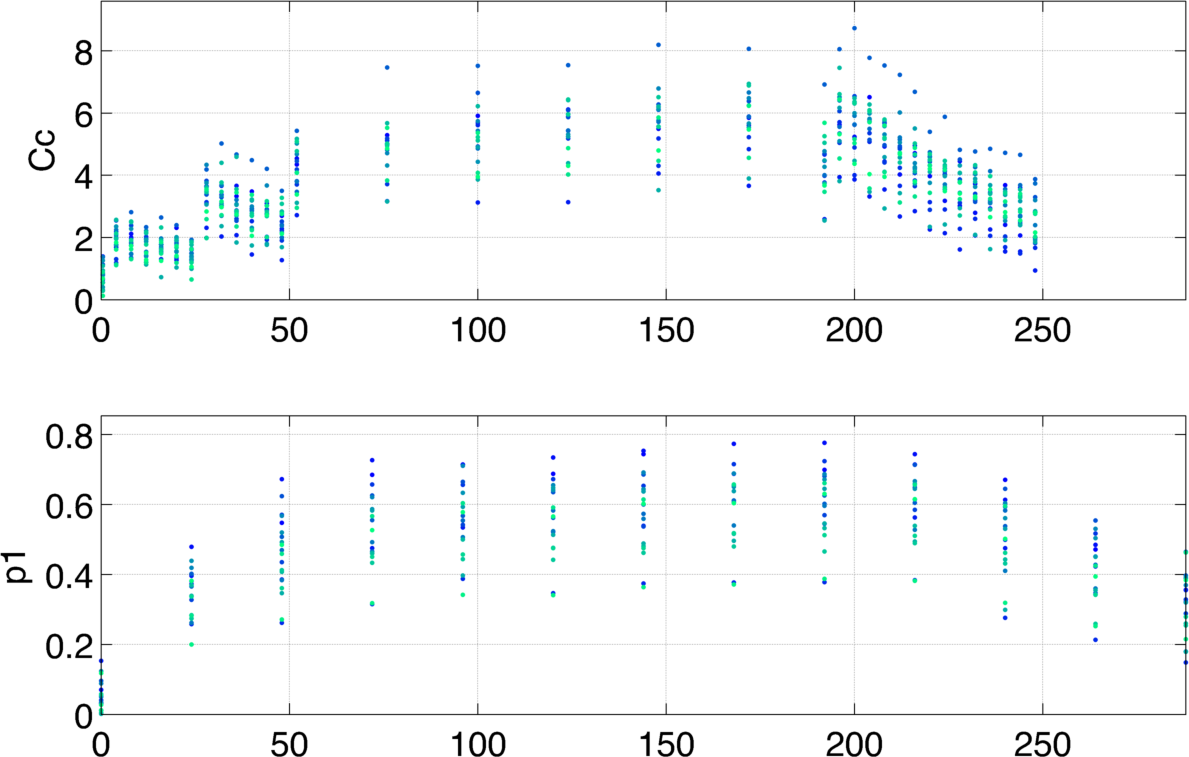
\includegraphics[width=.6\textwidth]{pics/p1_armA} 
\end{tabular}
\caption{Plots for first arm in the study. (top) Concentration, \emph{Cc}, time course of the PK model. 
(bottom) Probability, \emph{p1}, time course as defined in eq.\ref{eq:p1surface}.}
\label{fig:lambdasurface}
\end{figure}


%%%%%%%%%%%%%%%%%%%%%%%%%%%%%%%%%%%%%%%%%%%%%%%%%%%%%%%%%%%%%%%%
\subsection{Observation model}

\lstset{language=XML}
\begin{lstlisting}
        <ObservationModel blkId="om1">
            <Discrete>
                <CategoricalData ordered="no">
                    
                    <ct:Variable symbolType="real" symbId="p1">
                        <ct:Assign>
                            <math:Equation>
                                <math:Binop op="divide">
                                    <ct:Real>1</ct:Real>
                                    <math:Binop op="plus">
                                        <ct:Real>1</ct:Real>
                                        <math:Uniop op="exp">
                                            <math:Binop op="minus">
                                                <math:Uniop op="minus">
                                                    <ct:SymbRef blkIdRef="pm1" symbIdRef="theta1"/>
                                                </math:Uniop>
                                                <math:Binop op="times">
                                                    <ct:SymbRef blkIdRef="pm1" symbIdRef="theta2"/>
                                                    <math:Uniop op="log">
                                                        <ct:SymbRef blkIdRef="sm1" symbIdRef="Cc"/>
                                                    </math:Uniop>
                                                </math:Binop>
                                            </math:Binop>
                                        </math:Uniop>
                                    </math:Binop>
                                </math:Binop>
                            </math:Equation>                            
                        </ct:Assign>
                    </ct:Variable>
                    
                    <ListOfCategories> 
                        <Category symbId="cat0"/>
                        <Category symbId="cat1"/>
                    </ListOfCategories>
                    
                    <CategoryVariable symbId="y"/>
                    
                    <PMF linkFunction="identity">
                        <BinomialDistribution xmlns="http://www.uncertml.org/3.0" definition="">
                            <numberOfTrials>
                                <nVal>1</nVal>
                            </numberOfTrials>
                            <probabilityOfSuccess>
                                <var varId="p1"/>
                            </probabilityOfSuccess>
                        </BinomialDistribution>
                    </PMF>
                </CategoricalData>
            </Discrete>
        </ObservationModel>
\end{lstlisting}

%%%%%%%%%%%%%%%%%%%%%%%%%%%%%%%%%%%%%%%%%%%%%%%%%%%%%%%%%%%%%%%%
\subsection{NONMEM dataset}
\label{sec:eg7-NONMEMdataset}
The remaining part is the the data and trial design as sourced from the 
NONMEM dataset. Table \ref{tab:example7_dataSet} show a typical dataset required for 
an estimation task.
\begin{table}[htdp]
\begin{center}
\small
46	1	1
46	2	0
46	3	0
46	4	0
47	1	0
47	2	0
47	3	0
47	4	3
48	1	0
48	2	1
48	3	2
48	4	0
49	1	0
\renewcommand{\arraystretch}{1.1}% 
\begin{tabular}{rrrrrrrr}\toprule
ID 	& TIME	& AMT	& Y		& DVID \\ \midrule
1 	& 0 		& 100 	& . 		& . \\ 
1 	& 1 		& . 		& 1	 	& 2 \\ 
1 	& 4 		& . 		& 9.2 	& 1 \\ 
1 	& 8 		& . 		& 0 		& 2 \\ 
1 	& 10		& . 		& 0	 	& 2 \\ 
1 	& 12 	& . 		& 8.5 	& 1 \\ 
1 	& 18 	& . 		& 6.4 	& 1 \\ 
1 	& 24 	& . 		& 1 		& 2 \\ 
2 	& 0 		& 120	&  26 	& . \\ 
2 	& 4 		& . 		& 4.8 	& 1 \\ 
2 	& 8 		& . 		& 0 		& 2 \\ 
2 	& 12 	& . 		& 3.1 	& 1 \\ 
2 	& 18 	& . 		& 2.5 	& 1 \\ 
2 	& 24 	& . 		& 1 		& 2 \\ 
...	& ...		& ...		& ...		& ...	\\ \bottomrule
\end{tabular}
\end{center}
\caption{A dataset used in example for first two subjects.
The additional column DVID is used to specify the type of data. Here, 
DVID =1 is used for a continuous response and DVID =2 for count data.}
\label{tab:example7_dataSet}
\end{table}%

%%%%%%%%%%%%%%%%%%%%%%%%%%%%%%%%%%%%%%%%%%%%%%%%%%%%%%%%%%%%%%%%
\subsubsection{'Nested' mapping}

\lstset{language=XML}
\begin{lstlisting}
        <mstep:ExternalDataSet toolName="NONMEM" oid="NMoid">
            
            <mstep:ColumnMapping>
                <ds:ColumnRef columnIdRef="TIME"/>
                <ct:SymbRef symbIdRef="t"/>
            </mstep:ColumnMapping>
            <mstep:ColumnMapping>
                <ds:ColumnRef columnIdRef="AMT"/>
                <ct:SymbRef blkIdRef="sm1" symbIdRef="Ad"/>
            </mstep:ColumnMapping>
            <mstep:MultipleDVMapping>
                <ds:ColumnRef columnIdRef="DV"/>
                <mstep:Piecewise>
                    <math:Piece>
                        <ct:SymbRef blkIdRef="om1" symbIdRef="y"/>
                        <math:CategoryMapping>
                            <ds:Map dataSymbol="0" modelSymbol="cat0"/>
                            <ds:Map dataSymbol="1" modelSymbol="cat1"/>
                        </math:CategoryMapping>
                        <math:Condition>
                            <math:LogicBinop op="eq">
                                <ds:ColumnRef columnIdRef="DVID"/>
                                <ct:Int>2</ct:Int>
                            </math:LogicBinop>
                        </math:Condition>
                    </math:Piece>
                    <math:Piece>
                        <ct:SymbRef blkIdRef="om2" symbIdRef="C_obs"/>
                        <math:Condition>
                            <math:LogicBinop op="eq">
                                <ds:ColumnRef columnIdRef="DVID"/>
                                <ct:Int>1</ct:Int>
                            </math:LogicBinop>
                        </math:Condition>
                    </math:Piece>
                </mstep:Piecewise>
            </mstep:MultipleDVMapping>
            
            <!-- Dataset omitted, identical as in previous example -->
        </mstep:ExternalDataSet>
\end{lstlisting}



%%%%%%%%%%%%%%%%%%%%%%%%%%%%%%%%%%%%%%%%%%%%%%%%%%%%%%%%%%%%%%%%
%%%%%%%%%%%%%%%%%%%%%%%%%%%%%%%%%%%%%%%%%%%%%%%%%%%%%%%%%%%%%%%%
%%%%%%%%%%%%%%%%%%%%%%%%%%%%%%%%%%%%%%%%%%%%%%%%%%%%%%%%%%%%%%%%

\newpage

\eglabel{8}
\section{Example \theexamples: Joint PKPD model with Time-to-event effect}
\label{sec:eg8}

%%%%%%%%%%%%%%%%%%%%%%%%%%%%%%%%%%%%%%%%%%%%%%%%%%%%%%%%%%%%%%%%
\subsection{Description}
\label{subsec:exp8_intro} 
Time-to-effect is yet another type of discrete models supported by \pml, see Section 
\ref{subsec:DiscreteData} for detailed description.
In this example we consider a concentration dependent hazard function for which 
the cumulative hazard reads

\begin{eqnarray}
\frac{dCh}{dt} = hazard = \beta \times Cc(t) \quad \Longrightarrow \quad Ch(t) = \beta \int_0^{t} Cc(\tilde{t}) \;d\tilde{t} = \beta \times AUC(Cc(0,t))  \label{eq:hazardODE1}
\end{eqnarray}
The survival function reads, eq.\eqref{eq:survivalFct},
\begin{eqnarray}
S(t) = \exp(-Ch(t)) = \exp(- \beta \times AUC(Cc(0,t))) \label{eq:survivalFct}
\end{eqnarray}

\begin{figure}[htb!]
\centering
\begin{tabular}{cc}
 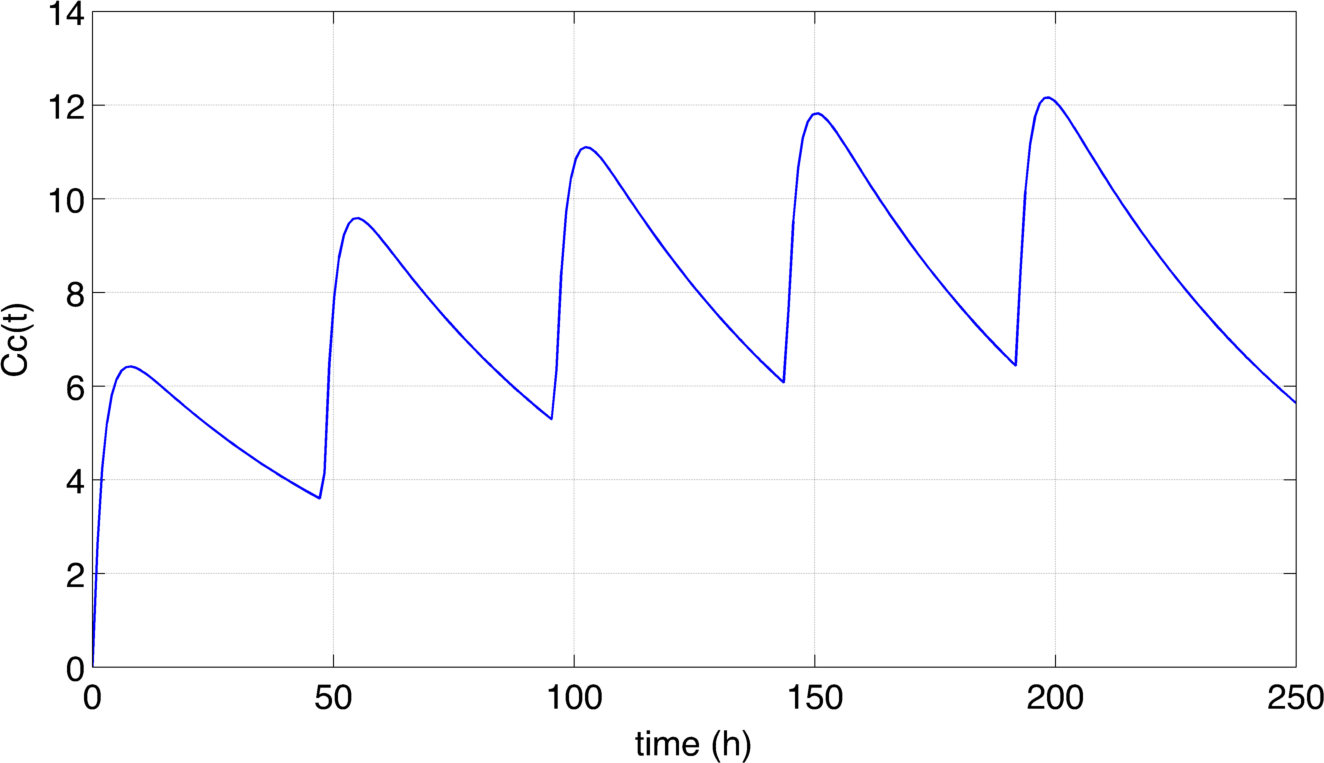
\includegraphics[width=70mm]{pics/example8_singleCc} & 
 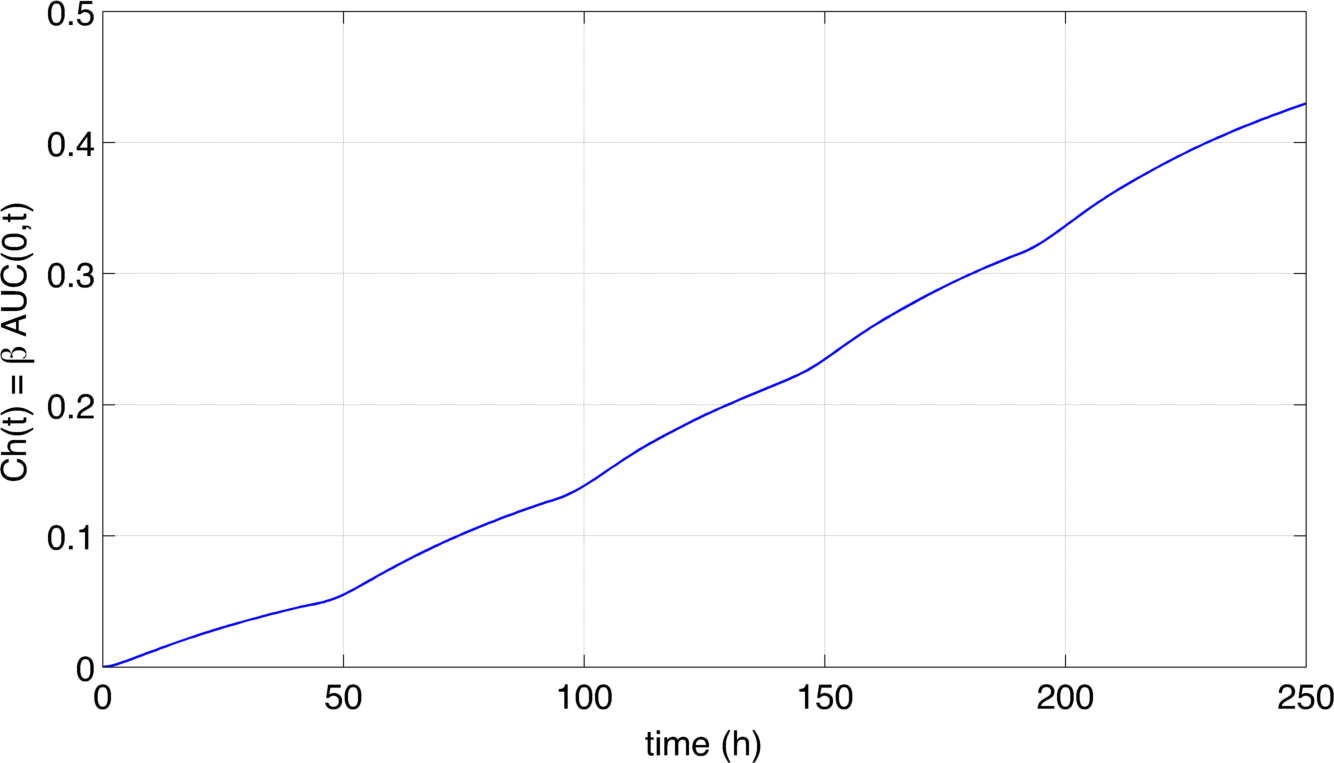
\includegraphics[width=70mm]{pics/example8_singleCh} \\
 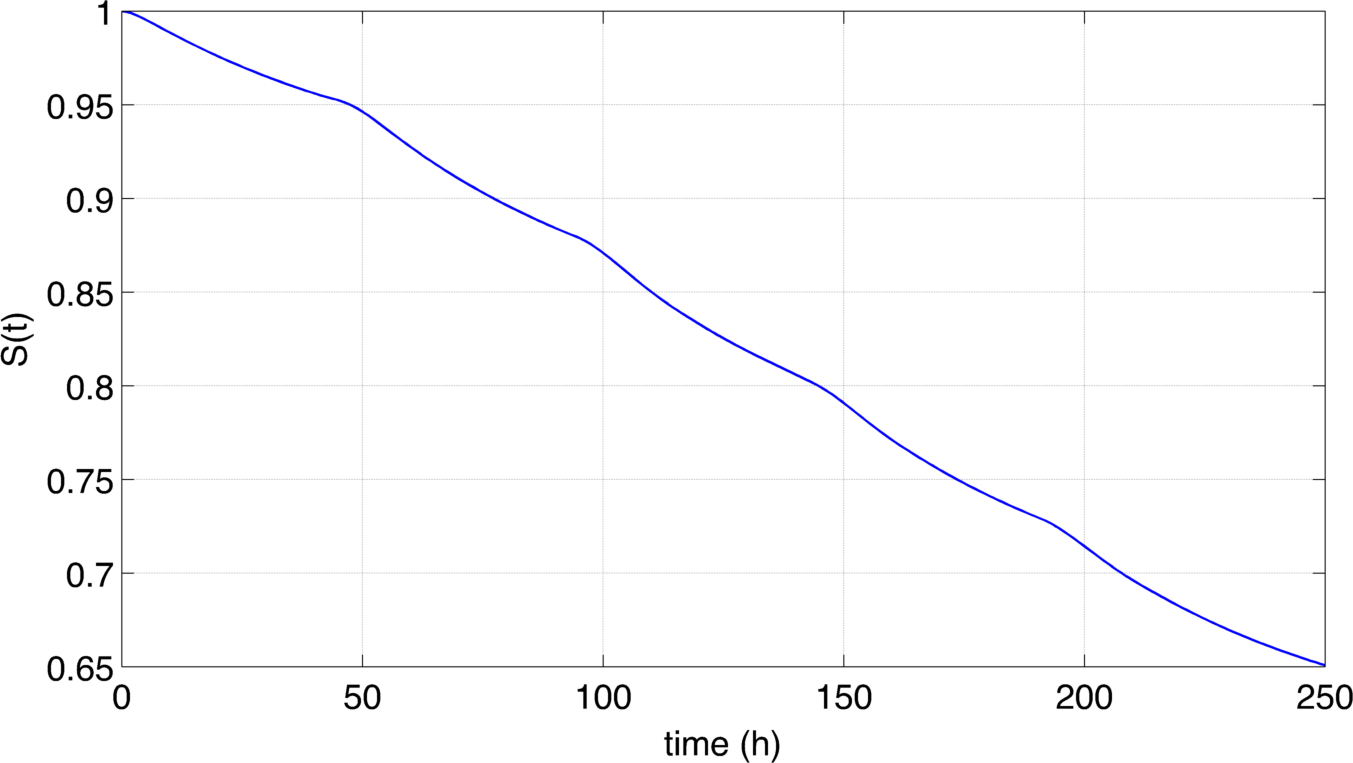
\includegraphics[width=70mm]{pics/example8_singleS} &
\end{tabular}
\caption{Single subject time course for concentration, \emph{Cc}, cumulative hazard, \emph{Ch}, 
and survival function, \emph{S}.}
\end{figure}


\subsubsection{Individual parameters model}
\begin{eqnarray}
beta& \sim&  \mbox{logNormal}(pop_{beta}, \omega_{beta}); \quad \pop_{beta}=0.13,\quad \omega_{beta}=0.2 \nonumber
\end{eqnarray}

\subsubsection{Observation model}
We apply a combined residual error model to the continuous PK output variable 
\var{Cc} and Poisson error distribution for the discrete PD component, defined by \var{Y}, 
as the following table shows 

%\begin{table*}[h!]
\begin{center}
\small
\renewcommand{\arraystretch}{1.1}% 
\begin{tabular*}{0.8\linewidth}{@{\extracolsep{\fill}} >{\bfseries}l l l}\toprule
Output Variable & \textbf{\itshape Cc} &\textbf{\itshape Y}\\\midrule
Observation Name & Concentration & State \\
Units & $\mg/l$ & -- \\
Type & Continuous & Discrete/Categorical \\
Model & Combined & Binomial\\
Parameters 	& $a, b$ 	& $\theta_1$, $\theta_2$\\
%Regressor	& --		& $Cc$ \\
\bottomrule
\end{tabular*}
\end{center}

%%%%%%%%%%%%%%%%%%%%%%%%%%%%%%%%%%%%%%%%%%%%%%%%%%%%%%%%%%%%%%%%
\subsubsection{Modelling Steps}

The PK and PD output variables to be generated by the simulation and
their associated time points are shown below:

\begin{center}
\small
\renewcommand{\arraystretch}{1.1}% 
\begin{tabular*}{0.9\linewidth}{@{\extracolsep{\fill}} >{\bfseries}l c c}\toprule
Output Variable & \textbf{\itshape Cc} &\textbf{\itshape $p1$}\\\midrule
Observation times & [0.5,4 : 4 : 48, 52 : 24 : 192, 192 : 4 : 250] & 0 : 24 : 288\\
\bottomrule
\end{tabular*}
\end{center}


%%%%%%%%%%%%%%%%%%%%%%%%%%%%%%%%%%%%%%%%%%%%%%%%%%%%%%%%%%%%%%%%
\subsection{Observation model}

\lstset{language=XML}
\begin{lstlisting}

\end{lstlisting}

%\begin{figure}
%\centering
%\begin{tabular}{cc}
% 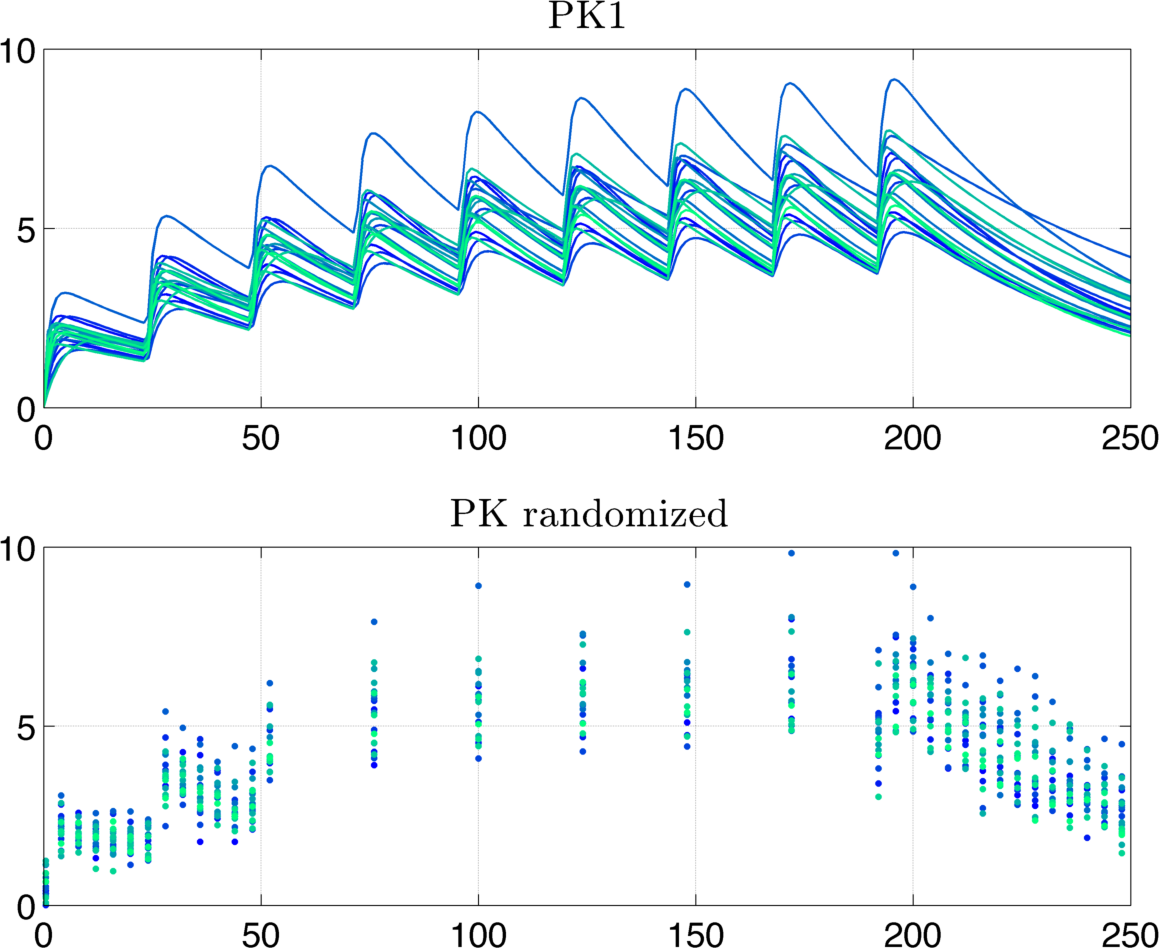
\includegraphics[width=80mm]{pics/example8_PK1_PK2} &
% 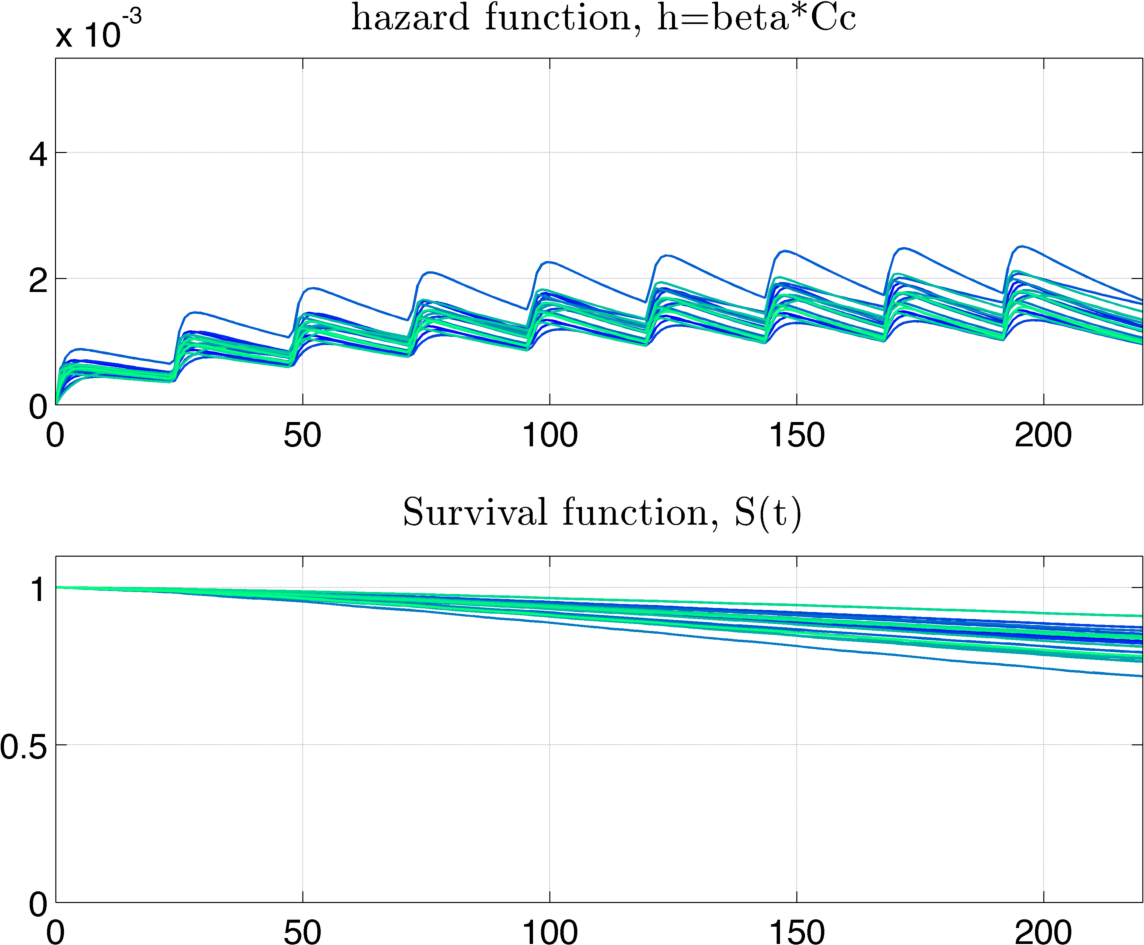
\includegraphics[width=80mm]{pics/example8_hazardPD_S}
%\end{tabular}
%\caption{PK as calculated from the PK model (top left) and with residual error model (bottom left). Hazard and survival function plot, here for arm A (right.)}
%\end{figure}


%%%%%%%%%%%%%%%%%%%%%%%%%%%%%%%%%%%%%%%%%%%%%%%%%%%%%%%%%%%%%%%%
\subsection{NONMEM dataset}
\label{sec:eg8-NONMEMdataset}
The remaining part is the the data and trial design as sourced from the 
NONMEM dataset. Table \ref{tab:example8_dataSet} show a typical dataset required for 
an estimation task.
\begin{table}[htdp]
\begin{center}
\small
\renewcommand{\arraystretch}{1.1}% 
\begin{tabular}{rrrrrrrr}\toprule
ID 	& TIME	& AMT	& Y		& DVID \\ \midrule
1 	& 0 		& 100 	& . 		& . \\ 
1 	& 1 		& . 		& 1	 	& 2 \\ 
1 	& 4 		& . 		& 9.2 	& 1 \\ 
1 	& 8 		& . 		& 0 		& 2 \\ 
1 	& 10		& . 		& 0	 	& 2 \\ 
1 	& 12 	& . 		& 8.5 	& 1 \\ 
1 	& 18 	& . 		& 6.4 	& 1 \\ 
1 	& 24 	& . 		& 1 		& 2 \\ 
2 	& 0 		& 120	&  26 	& . \\ 
2 	& 4 		& . 		& 4.8 	& 1 \\ 
2 	& 8 		& . 		& 0 		& 2 \\ 
2 	& 12 	& . 		& 3.1 	& 1 \\ 
2 	& 18 	& . 		& 2.5 	& 1 \\ 
2 	& 24 	& . 		& 1 		& 2 \\ 
...	& ...		& ...		& ...		& ...	\\ \bottomrule
\end{tabular}
\end{center}
\caption{A dataset used in example for first two subjects.
The additional column DVID is used to specify the type of data. Here, 
DVID =1 is used for a continuous response and DVID =2 for count data.}
\label{tab:example8_dataSet}
\end{table}%





